\documentclass[12pt, oneside]{book}
% -------------------
% --- usepackages ---
% -------------------
% \usepackage[utf8]{inputenc} % No necesario en LaTeX moderno (TeX Live 2018+)
\usepackage{amsfonts}
\usepackage{csquotes} % For "csquotes missing" warning and babel-biblatex compatibility
\usepackage[
	spanish
]{babel} % Bibliography
\usepackage[
	backend=biber,
	style=numeric,
	sorting=none,
	maxbibnames=99
]{biblatex} % Bibliography
\usepackage{amsmath} % For equations.
\usepackage{amsthm} % For theorem, definition, lemma and proofs.
\usepackage{siunitx} % To write degree symbol for angles.
\usepackage{graphicx} % To add images
\usepackage{xcolor} % To add pdf_tex images
\usepackage{import} % To add pdf_tex images
\usepackage{changepage} % To adjustwidth
\usepackage{multirow} % To merge cells in table
\usepackage[
	Algoritmo
]{algorithm} % To write Algorithms
\usepackage[
	noend
]{algpseudocode} % To write Algorithms
\usepackage{caption} % To add subfigures
\usepackage[
	list=true
]{subcaption} % To add subfigures
\usepackage{booktabs} % To change weight of table lines
\usepackage{imakeidx} % To make index
\usepackage{geometry} % To set margin and page size
\usepackage{setspace} % To set interline spacing
\usepackage{chngcntr} % To enumerate captions by chapter
\usepackage{hyperref} % To autogenerate hyperlinks
\usepackage{amssymb} % For \boxplus.
\usepackage{environ} % To define appendix command
\usepackage{mathrsfs} % To cursive font
\usepackage{titlesec} % For custom chapter heading style
\usepackage{enumitem} % To define new type of list
\usepackage{multicol} % For multiple column in one page
\usepackage{cleveref} % For footnotes in multiple sentences

% -------------------------
% --- makeindex options ---
% -------------------------
%     title:        header title
%     options= -s:  .ist file
%     intoc:        add to table of content
\makeindex[title=ÍNDICE ALFABÉTICO, options= -s index.ist, intoc]

% -------------------------
% --- bibliography file ---
% -------------------------
\addbibresource{bibliography.bib}

% ----------------------------
% --- document information ---
% ----------------------------
\title{Complejidad Computacional de Problemas de Empaquetamiento con Trominós}
\author{Javier Tadashi Akagi Fukushima}
\date{September 2019}

% -----------------------------
% --- page size and margins ---
% -----------------------------
\geometry{
	a4paper, 
	tmargin = 2.5cm,
	bmargin = 2cm,
	rmargin = 1.5cm,
	lmargin = 2.5cm
}

% ---------------------------------
% --- page format and numbering ---
% ---------------------------------
\pagestyle{plain}

% -----------------------
% --- interline space ---
% -----------------------
\onehalfspacing
%\spacing{1.5}
%\doublespacing

% --------------------------------
% --- font style               ---
% ---  of definition, theorems ---
% --------------------------------
%     definition style: roman
\theoremstyle{definition}

% -------------------------
% --- caption numbering ---
% -------------------------
%     numbering by chapter:
%     <number of chapter>.<number of figure>
\counterwithin{figure}{chapter}
\counterwithin{equation}{chapter}
\counterwithin{table}{chapter}
\counterwithin{algorithm}{chapter}

% ----------------------------
% --- caption label format ---
% ----------------------------
%     subfigure caption format:
%     (<subfigure enumeration>) <description>
%\DeclareCaptionLabelFormat{subfigure}{Figura#1~\thefigure(#2):}
\DeclareCaptionLabelFormat{subfigureComment}{(#2):}
\DeclareCaptionLabelFormat{subfigureOnlyNumber}{(#2)}
%\DeclareCaptionLabelFormat{noCaption}{}
%\captionsetup[sub]{labelformat=subfigure}
\captionsetup[sub]{labelformat=subfigureOnlyNumber}

% ----------------------------------------
% --- table of content, list of figure ---
% ---  and list of table reedefinition ---
% ----------------------------------------
%     <title>                         Page
%     1. <chapter title> .... <page number>

\makeatletter
\renewcommand\tableofcontents{%
	\noindent
	\textbf{\large ÍNDICE} \hspace*{\fill} Página
	
	\@starttoc{toc}%
}
\makeatother

\makeatletter
\renewcommand\listoffigures{%
	\noindent
	\textbf{\large LISTA DE FIGURAS} \hspace*{\fill} Página

    \@starttoc{lof}%
}
\makeatother

\makeatletter
\renewcommand\listoftables{%
	\noindent
	\textbf{\large LISTA DE TABLAS} \hspace*{\fill} Página

    \@starttoc{lot}%
}
\makeatother

% ---------------------------
% --- new list definition ---
% ---------------------------
\newlist{listsymbol}{itemize}{1}
\setlist[listsymbol,1]{
	label=,
	labelwidth=1.9cm,
	align=parleft,
	itemsep=0.1\baselineskip,
	leftmargin=!
}

% ----------------------
% --- newenvironment ---
% ----------------------
\newenvironment{proofidea}{\begin{proof}[La idea de la demostración]}{\end{proof}}
\newenvironment{blockindent}{\vskip 0cm
\begin{adjustwidth}{.5cm}{.5cm}}{\end{adjustwidth}
\vskip .5cm}

% ------------------
% --- newcommand ---
% ------------------
\newcommand{\aztecdiam}{\mathcal{AD}} % To denote AD (aztec diamond)
\newcommand{\aztecrect}{\mathcal{AR}} % To denote AR (aztec rectangle)

\newcommand{\midbar}{\;\middle|\;} % To draw midline in set

\newcommand{\inout}[3]{ % To write a problem statement
	\vspace{0.2cm}
	\noindent
	\begin{tabular}{p{.13\textwidth} p{.006\textwidth} p{.775\textwidth}}
		\multicolumn{3}{l}{\scalebox{.85}{\textsc{#1}}}\\
		\hline
		\multicolumn{1}{|l}{ENTRADA} &:& \multicolumn{1}{p{.775\textwidth}|}{#2} \\
		\multicolumn{1}{|l}{SALIDA} &:& \multicolumn{1}{p{.775\textwidth}|}{#3} \\
		\hline
	\end{tabular}
	\vspace{0.2cm}
}
% \inout{<title>}{<input statement>}{<output statement>}
%
% will produce:
%
%  <title>
%  /--------------------------------\
%  | ENTRADA : <input statement>    |
%  | SALIDA  : <output statement>   |
%  \--------------------------------/

% -------------------------------------
% --- custom chapter heading format ---
% -------------------------------------
%     Label:  Chapter <chapter number>
%     Title:  <chapter title>
\newcommand{\chapterformatdefault}{
	\titleformat{\chapter}[display]
		{\LARGE } % Format for Label and Title
		{\vspace*{3.5cm}\MakeUppercase{\chaptertitlename} {\thechapter}} % Label
		{.2 cm} % Horizontal separation
		{\bfseries } % Code preceding to title body.
}

%     Title:  <chapter title>
\newcommand{\chapterformattitleonly}{
	\titleformat{\chapter}[display]
		{\LARGE } % Format for Label and Title
		{\vspace*{3.5cm}\MakeUppercase{\chaptertitlename} {\thechapter}} % Label
		{.2 cm} % Horizontal separation
		{\bfseries } % Code preceding to title body.
}

\newcommand{\trominodl}{\begin{gathered}\includegraphics[scale=.75]{images/L-tromino1.pdf}\end{gathered}} % To write a L-tromino in equation.
\newcommand{\trominodr}{\begin{gathered}\includegraphics[scale=.75]{images/L-tromino2.pdf}\end{gathered}} % To write a L-tromino in equation.
\newcommand{\trominour}{\begin{gathered}\includegraphics[scale=.75]{images/L-tromino3.pdf}\end{gathered}} % To write a L-tromino in equation.
\newcommand{\trominoul}{\begin{gathered}\includegraphics[scale=.75]{images/L-tromino4.pdf}\end{gathered}} % To write a L-tromino in equation.
\newcommand{\dominov}{\begin{gathered}\includegraphics[scale=.75]{images/dominoV.pdf}\end{gathered}} % To write a domino in equation.
\newcommand{\dominoh}{\begin{gathered}\includegraphics[scale=.75]{images/dominoH.pdf}\end{gathered}} % To write a domino in equation.
\newcommand{\floor}[1]{\left \lfloor #1 \right \rfloor} % To denote floor function

\newcommand\blfootnote[1]{ % To generate a footnote without marker
	\begingroup
	\renewcommand\thefootnote{}\footnote{#1}%
	\addtocounter{footnote}{-1}%
	\endgroup
}

% ---------------------------
% --- spanish translation ---
% ---------------------------

% -- Spanish theorems ---
\newtheorem{theorem}{Teorema}
\numberwithin{theorem}{chapter} % To number theorems according to the chapter
\newtheorem{definition}{Definición}
\numberwithin{definition}{chapter} % To number definitions according to the chapter
\newtheorem{lemma}{Lema}
\numberwithin{lemma}{chapter} % To number lemmas according to the chapter
\newtheorem{corollary}{Corolario}
\numberwithin{corollary}{chapter} % To number corollaries according to the chapter
\newtheorem{example}{Ejemplo}
\numberwithin{example}{chapter} % To number examples according to the chapter
\newtheorem{openproblem}{Problema abierto}
\numberwithin{openproblem}{chapter} % To number open problem according to the chapter
\addto\spanish{\renewcommand\proofname{Demostración}}

% -- Spanish algorithmic --
\algdef{S}[FOR]{ForEach}[1]{\algorithmicforeach\ #1\ \algorithmicdo}
\algnewcommand\algorithmicforeach{\textbf{para cada}}

\renewcommand{\algorithmicprocedure}{\textbf{procedimiento}}
\renewcommand{\algorithmicend}{\textbf{fin}}
\renewcommand{\algorithmicif}{\textbf{si}}
\renewcommand{\algorithmicthen}{\textbf{entonces}}
\renewcommand{\algorithmicelse}{\textbf{sino }}
\renewcommand{\algorithmicfor}{\textbf{desde}}
\renewcommand{\algorithmicforall}{\textbf{para todo}}
\renewcommand{\algorithmicdo}{\textbf{repetir}}
\renewcommand{\algorithmicwhile}{\textbf{mientras}}
\renewcommand{\algorithmicrepeat}{\textbf{repetir}}
\renewcommand{\algorithmicuntil}{\textbf{antes de}}
\renewcommand{\algorithmicreturn}{\textbf{retornar}}
%\renewcommand{\algorithmicrequire}{\textbf{Require:}}
%\renewcommand{\algorithmicensure}{\textbf{Ensure:}}
%\renewcommand{\algorithmicelsif}{\algorithmicelse\ \algorithmicif}
%\renewcommand{\algorithmicendif}{\algorithmicend\ \algorithmicif}
%\renewcommand{\algorithmicendfor}{\algorithmicend\ \algorithmicfor}
%\renewcommand{\algorithmicendwhile}{\algorithmicend\ \algorithmicwhile}
%\renewcommand{\algorithmicloop}{\textbf{loop}}
%\renewcommand{\algorithmicendloop}{\algorithmicend\ \algorithmicloop}

% -- Spanish list title --
\addto\captionsspanish{\renewcommand*\contentsname{ÍNDICE}}
\addto\captionsspanish{\renewcommand*\listfigurename{LISTA DE FIGURAS}}
\addto\captionsspanish{\renewcommand*\listtablename{LISTA DE TABLAS}}


\setcounter{secnumdepth}{5}

\begin{document}

\frontmatter

% -- Portada --
\thispagestyle{empty}

\vspace{2.5cm}

\noindent
\centerline{\textsc{\Large Universidad Nacional de Asunción}}
\centerline{\textsc{\Large Facultad Politécnica}}

\vspace{1cm}

\noindent
\centerline{\textsc{\large Ingeniería en Informática}}

\vspace{1cm}

\centerline{
\includegraphics[scale=.4]{images/logo_fpuna}}


\vspace{2.5cm}

\centerline{\textbf{\large Detección de familias de ransomware en base a}}
\centerline{\textbf{\large archivos encriptados y notas de rescate}}

\vspace{4cm}

\centerline{\small \textbf{Romina Alfonzo}}
\centerline{\small \textbf{Carlos Urdapilleta}}

\vspace{1cm}

\centerline{Proyecto de Trabajo de Grado presentado en conformidad a los}
\centerline{requisitos para obtener el grado de XXXXXX}


\vspace*{\fill}

\centerline{San Lorenzo - Paraguay}
\centerline{XXXXXX - 2024}

\vspace{3cm}


% -- Página de cortesía --
\newpage
\thispagestyle{empty}
\null
\clearpage 
	
% -- Carátula --
\newpage
\setcounter{page}{1}
\thispagestyle{empty}

\vspace{2.5cm}

\noindent
\centerline{\textsc{\large Universidad Nacional de Asunción}}
\centerline{\textsc{\large Facultad Politécnica}}

\vspace{1cm}

\noindent
\centerline{\textsc{\large Carrera}}

\vspace{1cm}

\centerline{
\includegraphics[scale=.4]{images/logo_fpuna}}

\vspace{1.5cm}

\centerline{\textbf{Titulo 1}}
\centerline{\textbf{Titulo 2}}

\vspace*{\fill}

\centerline{\small \textbf{Nombre y apellido}}

\vspace*{\fill}

\centerline{San Lorenzo - Paraguay}
\centerline{Septiembre - 2019}

\vspace{2.5cm}


% -- Título --
\newpage
\thispagestyle{empty}

\vspace{2.5cm}

\noindent
\centerline{\textsc{\large Universidad Nacional de Asunción}}
\centerline{\textsc{\large Facultad Politécnica}}

\vspace{1cm}

\noindent
\centerline{\textsc{\large Carrera}}

\vspace{1cm}

\centerline{
\includegraphics[scale=.4]{images/logo_fpuna}}

\vspace{1.5cm}

\centerline{\textbf{Titulo 1}}
\centerline{\textbf{Titulo 2}}

\vspace{1cm}


\vspace{1cm}

\centerline{\small \textbf{Nombre completo}}

\vspace{1.5cm}

Asesor:

\hspace{1cm} Supervisor

\vspace{2cm}

\centerline{Proyecto de Trabajo de Grado/Maestria/Doctorado presentado en conformidad a los}
\centerline{requisitos para obtener el grado de XXXXXXX}




\vspace*{\fill}

\centerline{San Lorenzo - Paraguay}
\centerline{Septiembre - 2019}

\vspace{2.5cm}




% -- Hoja de aprobación --
%\newpage
%\input{aprobacion.tex}

% -- Dedicatoria --
\newpage
\input{dedicatoria.tex}

% -- Agradecimientos --
\newpage
\input{agradecimientos.tex}

% -- Resumen --
\newpage
\input{resumen_es.tex}

% -- Summary --
\newpage
\input{resumen_en.tex}


% -- Índice --
%(Indice o Contenido (?) )
\newpage
\tableofcontents

% -- Lista de figuras --
\newpage
\listoffigures
 
% -- Lista de tablas --
\newpage
\listoftables

% -- Lista de símbolos --
\newpage
\input{lista_simbolos.tex}

% ----------------------------------------------
% ----------------------------------------------
% ----------------------------------------------

\mainmatter
\chapterformatdefault

% ------------------
% -- INTRODUCCIÓN --
% ------------------
\chapter{INTRODUCCIÓN}
\thispagestyle{empty}
\section{Contexto y Motivación}

El ransomware representa una de las amenazas cibernéticas más significativas de la última década, con pérdidas económicas globales estimadas en miles de millones de dólares anuales~\cite{europol2023}. Este tipo de malware restringe el acceso a los datos de la víctima mediante la encriptación de archivos y exige un pago, generalmente en criptomonedas, para restaurar el acceso. A diferencia de otras formas de malware que buscan robar información o comprometer sistemas de manera encubierta, el ransomware confronta directamente a la víctima con la pérdida de sus datos.

Si bien la investigación en ransomware ha sido extensa en términos de prevención y detección temprana, el análisis post-ataque ha recibido considerablemente menos atención~\cite{paper_4_comparison_of_entropy}. La mayoría de las investigaciones se centran en el análisis del ejecutable malicioso, un enfoque que resulta poco práctico en escenarios reales donde el atacante suele eliminar el binario tras completar la encriptación. En contraste, los artefactos que invariablemente permanecen después de un ataque son los archivos encriptados y las notas de rescate depositadas por el ransomware.

La identificación de la familia de ransomware responsable de un ataque constituye un paso crítico en la respuesta a incidentes, ya que permite determinar si existen herramientas de descifrado disponibles, evaluar la probabilidad de recuperación de datos, y caracterizar el modus operandi del grupo atacante. Herramientas existentes como CryptoSheriff e ID Ransomware abordan parcialmente este problema, pero presentan limitaciones significativas: CryptoSheriff clasifica correctamente solo el 16,67\% de las familias de ransomware, mientras que ID Ransomware alcanza el 66,67\% utilizando archivos encriptados, y el 72\% cuando se emplean notas de rescate~\cite{paper_2_on_efectiveness}.

Estos resultados revelan una brecha importante en la capacidad de identificación automatizada de familias de ransomware, y sugieren que las notas de rescate contienen información discriminativa valiosa que no está siendo explotada adecuadamente por los métodos actuales.

\section{Planteamiento del Problema}

El problema central que aborda este trabajo es la clasificación automatizada de familias de ransomware en un escenario post-ataque, donde los únicos artefactos disponibles son los archivos encriptados y las notas de rescate.

Este problema presenta dos desafíos fundamentales. El primero se relaciona con la naturaleza de los archivos encriptados: los algoritmos criptográficos modernos (AES, RSA, ChaCha20) producen salidas estadísticamente indistinguibles de datos aleatorios~\cite{paper_4_comparison_of_entropy, paper_3_enhancing_file_entropy}. Esto implica que las métricas estadísticas tradicionales como la entropía de Shannon, si bien son efectivas para detectar la presencia de encriptación, resultan insuficientes para discriminar entre diferentes familias de ransomware. Trabajos recientes han demostrado que la entropía de Shannon no es la métrica óptima para todos los escenarios de detección, y que la combinación de múltiples pruebas estadísticas, incluyendo Chi-Cuadrado, Monte Carlo y el coeficiente de correlación serial de bytes, ofrece resultados superiores en la detección de archivos cifrados~\cite{lee2022}.

El segundo desafío concierne a las notas de rescate: aunque cada familia de ransomware utiliza plantillas de texto características, la recopilación de un corpus suficientemente amplio y representativo de estas notas constituye un problema abierto, dado que no existe un repositorio centralizado y estandarizado.

\section{Objetivos}

\subsection{Objetivo General}

Evaluar y comparar técnicas de aprendizaje automático para la clasificación de familias de ransomware utilizando dos fuentes de evidencia post-ataque: las propiedades estadísticas de archivos encriptados y el análisis de procesamiento de lenguaje natural (NLP) de notas de rescate.

\subsection{Objetivos Específicos}

\begin{enumerate}
    \item Evaluar la efectividad de métricas estadísticas (entropía de Shannon, Chi-Cuadrado, estimación Monte Carlo de $\pi$, coeficiente de correlación serial de bytes) para la detección binaria de archivos cifrados por ransomware versus archivos seguros, utilizando el dataset NapierOne.

    \item Investigar las limitaciones de la clasificación multiclase de familias de ransomware basada exclusivamente en propiedades estadísticas de archivos encriptados, proporcionando evidencia empírica de la indistinguibilidad estadística entre familias.

    \item Construir un corpus de notas de rescate asociadas a las 30 familias de ransomware del dataset NapierOne, integrando múltiples fuentes públicas.

    \item Implementar y evaluar un sistema de clasificación de familias de ransomware basado en el análisis NLP de notas de rescate, utilizando técnicas de TF-IDF y modelos de aprendizaje automático.

    \item Comparar cuantitativamente la efectividad de ambos enfoques (análisis de archivos vs. análisis de notas) para la identificación de familias de ransomware.
\end{enumerate}

\section{Alcance y Limitaciones}

El presente trabajo se enfoca en 30 familias de ransomware incluidas en el dataset NapierOne~\cite{paper_7_napierone}, que abarca variantes activas entre 2013 y 2022. El análisis de archivos encriptados se realiza sobre las versiones \textit{extra-small} y \textit{small} del dataset, que contienen 100 y 1.000 archivos por familia respectivamente, además de archivos seguros pertenecientes a 44 tipos de archivos comunes.

Para el corpus de notas de rescate, se integran muestras provenientes de repositorios públicos (ThreatLabz~\cite{threatlabz}, Lemmou~\cite{paper_5_dataset}) y notas documentadas en reportes de seguridad de fuentes reconocidas (CISA, Securelist, BleepingComputer, CrowdStrike).

Las principales limitaciones del trabajo incluyen: (a) la dependencia de datasets públicos que pueden no representar todas las variantes de cada familia; (b) la cantidad limitada de notas de rescate disponibles para algunas familias; (c) el enfoque restringido a archivos encriptados en reposo, sin considerar tráfico de red ni comportamiento dinámico del malware.

\section{Organización del Documento}

El presente documento se organiza de la siguiente manera. El Capítulo~2 presenta el marco teórico, incluyendo los fundamentos de ransomware, las métricas estadísticas empleadas, los algoritmos de aprendizaje automático seleccionados, las técnicas de procesamiento de lenguaje natural, y una revisión de los trabajos relacionados. El Capítulo~3 describe la metodología adoptada, detallando la preparación de datos, la extracción de características, y el diseño experimental. El Capítulo~4 presenta los resultados experimentales obtenidos en los tres escenarios evaluados (detección binaria, clasificación multiclase por archivos, y clasificación por notas de rescate), junto con un análisis comparativo. Finalmente, el Capítulo~5 recoge las conclusiones del trabajo, las contribuciones realizadas, y las líneas de trabajo futuro identificadas.

% -------------------
% -- MARCO TEÓRICO --
% -------------------
\chapter{MARCO TEÓRICO}
\thispagestyle{empty}
\section{Ransomware: Definición y Taxonomía}

El ransomware es un tipo de software malicioso que restringe el acceso a los datos o sistemas de la víctima y demanda un pago para restablecer dicho acceso. Se distinguen dos categorías principales: el \textit{crypto-ransomware}, que cifra archivos individuales utilizando algoritmos criptográficos, y el \textit{locker-ransomware}, que bloquea el acceso al sistema operativo sin necesariamente cifrar archivos~\cite{europol2023}.

El presente trabajo se enfoca en el \textit{crypto-ransomware}, dado que constituye la variante predominante en ataques modernos y genera los artefactos de interés: archivos encriptados y notas de rescate. Las 30 familias analizadas en este estudio, provenientes del dataset NapierOne~\cite{paper_7_napierone}, abarcan un amplio espectro temporal y técnico, desde CryptoLocker (2013) hasta BlackBasta (2022), e incluyen tanto operaciones de Ransomware-as-a-Service (RaaS) como grupos independientes.

\section{Dataset NapierOne}

El dataset NapierOne, desarrollado por Davies et al.~\cite{paper_7_napierone}, constituye el conjunto de datos de referencia utilizado en este trabajo para la evaluación de técnicas de detección y clasificación de ransomware. A diferencia de datasets anteriores basados en muestras ejecutables recopiladas de repositorios como VirusTotal~\cite{VirusTotal} o VirusShare~\cite{VirusShare}, NapierOne se enfoca en los \textit{archivos resultantes} de la encriptación, proporcionando un escenario realista de análisis post-ataque.

El dataset se estructura en tres niveles de escala:

\begin{itemize}
    \item \textbf{Extra-Small (Tiny):} 100 archivos encriptados por cada una de las 30 familias de ransomware, más 100 archivos seguros por cada uno de los 44 tipos de archivo comunes. Total aproximado: 7.400 archivos.
    \item \textbf{Small:} 1.000 archivos por familia y tipo. Total aproximado: 74.000 archivos.
    \item \textbf{Total:} 5.000 archivos por familia y tipo. Total aproximado: 370.000 archivos.
\end{itemize}

Las 30 familias de ransomware incluidas son: Avoslocker, BadRabbit, BlackBasta, BlackCat (ALPHV), BlackMatter, Cerber, Chimera, Clop, Conti, CryptoLocker, Cuba, DarkSide, Dharma, GandCrab, HelloKitty, Jigsaw, LockBit, Lorenz, Maze, MedusaLocker, Netwalker, NotPetya, Phobos, RansomEXX, Ryuk, Sodinokibi (REvil), SunCrypt, TeslaCrypt, WannaCry y WastedLocker.

Los archivos seguros cubren 44 formatos, agrupados en categorías como documentos de oficina, imágenes, audio, video, archivos comprimidos, ejecutables y bases de datos, representando los tipos de archivo más comúnmente encontrados en entornos corporativos y personales.

\section{Métricas Estadísticas para el Análisis de Archivos}

El análisis de las propiedades estadísticas de los archivos constituye el primer enfoque evaluado en este trabajo. Esta sección describe las métricas empleadas, fundamentando teóricamente su relevancia para la detección de encriptación.

\subsection{Entropía de Shannon}

La entropía de Shannon~\cite{shannon1948}, concepto seminal de la teoría de la información, cuantifica la incertidumbre inherente a una distribución de datos. Para un archivo considerado como secuencia de bytes, la entropía se calcula mediante:

\begin{equation}
    H(X) = -\sum_{i=0}^{255} P(x_i) \log_2 P(x_i)
\end{equation}

donde $P(x_i)$ representa la probabilidad empírica de ocurrencia del byte $x_i$. Los valores resultantes se encuentran en el rango $[0, 8]$, donde valores cercanos a 0 indican datos altamente predecibles y valores próximos a 8 sugieren máxima aleatoriedad.

Si bien la entropía de Shannon es ampliamente utilizada en la detección de ransomware, trabajos recientes han identificado limitaciones importantes. Lee et al.~\cite{lee2022} demostraron que la entropía de Shannon por sí sola no es la métrica óptima para todos los escenarios, presentando falsos positivos significativos con archivos comprimidos (ZIP, GZIP, MP4) que también exhiben valores de entropía cercanos a 8. Davies et al.~\cite{paper_4_comparison_of_entropy} confirmaron que, si bien la combinación de entropía alta con valores de $\chi^2$ que no rechazan uniformidad constituye un indicador fuerte de encriptación, la entropía por sí sola resulta insuficiente para distinguir entre archivos cifrados y archivos comprimidos nativamente.

\subsection{Prueba Chi-Cuadrado}

La prueba $\chi^2$ ofrece un marco estadístico formal para evaluar si la distribución observada de bytes se desvía significativamente de la uniformidad esperada en archivos encriptados. El estadístico se calcula como:

\begin{equation}
    \chi^2 = \sum_{i=0}^{255} \frac{(F_i - f_i)^2}{f_i}
\end{equation}

donde $F_i$ denota la frecuencia observada del byte $i$ y $f_i = \frac{N}{256}$ representa la frecuencia esperada bajo la hipótesis de uniformidad, siendo $N$ el número total de bytes. La interpretación requiere comparar el valor calculado con los valores críticos de la distribución $\chi^2$ con 255 grados de libertad.

Como señalan Davies et al.~\cite{paper_4_comparison_of_entropy}, la combinación de entropía alta con valores bajos de $\chi^2$ proporciona un indicador más robusto de encriptación que cualquiera de las métricas individualmente, ya que archivos comprimidos típicamente exhiben valores de $\chi^2$ que rechazan la hipótesis de uniformidad a pesar de tener entropía alta.

\subsection{Estimación Monte Carlo de \texorpdfstring{$\pi$}{pi}}

Esta métrica, derivada de la suite de pruebas estadísticas propuesta por Davies et al.~\cite{paper_4_comparison_of_entropy}, utiliza pares consecutivos de bytes del archivo como coordenadas $(x, y)$ en un espacio unitario para estimar el valor de $\pi$. El principio subyacente es que datos verdaderamente aleatorios producirán estimaciones que convergen al valor real de $\pi$:

\begin{equation}
    \hat{\pi} = 4 \cdot \frac{\text{puntos dentro del círculo unitario}}{\text{total de puntos}}
\end{equation}

Desviaciones significativas del valor esperado de $\pi$ sugieren patrones estructurales en los datos que son inconsistentes con la aleatoriedad pura generada por algoritmos criptográficos robustos.

\subsection{Coeficiente de Correlación Serial de Bytes (SBCC)}

El coeficiente de correlación serial evalúa la dependencia estadística entre bytes consecutivos en un archivo:

\begin{equation}
    r = \frac{n\sum_{i=1}^{n-1} x_i x_{i+1} - \left(\sum_{i=1}^{n} x_i\right)^2}{n\sum_{i=1}^{n} x_i^2 - \left(\sum_{i=1}^{n} x_i\right)^2}
\end{equation}

donde $x_i$ representa el valor del $i$-ésimo byte y $n$ la longitud del archivo. Para datos verdaderamente aleatorios, el coeficiente tiende a 0, indicando ausencia de correlación. Valores significativamente distintos de 0 sugieren patrones secuenciales que pueden revelar la presencia de estructuras de archivo no aleatorias~\cite{lee2022}.

Davies et al.~\cite{paper_4_comparison_of_entropy} encontraron que este coeficiente es particularmente útil como complemento de la entropía de Shannon, ya que permite distinguir archivos comprimidos (que exhiben cierta correlación serial) de archivos genuinamente cifrados (que presentan correlación cercana a cero).

\section{Algoritmos de Aprendizaje Automático}

En el presente estudio se evaluaron diversos algoritmos de aprendizaje automático para abordar tanto el problema de clasificación binaria (cifrado vs. seguro) como el de clasificación multiclase (identificación de familias). La selección de algoritmos busca cubrir un espectro amplio de enfoques: modelos lineales, métodos basados en instancias, y métodos de ensamblaje.

\subsection{Regresión Logística}

La regresión logística estima la probabilidad de pertenencia a una clase mediante la función logística:

\begin{equation}
    P(y = 1|\mathbf{x}) = \frac{1}{1 + e^{-(\beta_0 + \boldsymbol{\beta}^T \mathbf{x})}}
\end{equation}

donde $\beta_0$ es el intercepto y $\boldsymbol{\beta}$ el vector de coeficientes. Su interpretabilidad directa y eficiencia computacional la hacen adecuada como modelo base de comparación~\cite{hastie2009}.

\subsection{Máquinas de Soporte Vectorial (SVM)}

Las SVM formulan la clasificación como la optimización del margen entre clases:

\begin{equation}
    \min_{\mathbf{w},b} \frac{1}{2}\|\mathbf{w}\|^2 \quad \text{sujeto a} \quad y_i(\mathbf{w}^T\mathbf{x}_i + b) \geq 1 \quad \forall i
\end{equation}

Para el análisis de notas de rescate, se emplea la variante LinearSVC, particularmente efectiva en espacios de alta dimensionalidad como los generados por TF-IDF, donde el número de características supera ampliamente el número de muestras~\cite{joachims1998}.

\subsection{K-Nearest Neighbors (KNN)}

El algoritmo KNN realiza predicciones por votación mayoritaria entre los $k$ vecinos más cercanos:

\begin{equation}
    \hat{y} = \text{mode}(\{y_i | \mathbf{x}_i \in N_k(\mathbf{x}_q)\})
\end{equation}

Su naturaleza no paramétrica lo hace flexible ante distribuciones arbitrarias de datos, aunque su rendimiento depende críticamente de la normalización de características y la elección de la métrica de distancia~\cite{hastie2009}.

\subsection{Árboles de Decisión}

Los árboles de decisión particionan recursivamente el espacio de características maximizando la ganancia de información:

\begin{equation}
    IG(D_p, f) = I(D_p) - \sum_{j=1}^{m} \frac{N_j}{N_p} I(D_j)
\end{equation}

donde $I(\cdot)$ puede ser la impureza de Gini o la entropía informacional. Su principal ventaja es la interpretabilidad visual directa de las reglas de decisión aprendidas~\cite{breiman1984}.

\subsection{Random Forest}

Random Forest combina $B$ árboles de decisión entrenados mediante bagging y selección aleatoria de características:

\begin{equation}
    \hat{f}(\mathbf{x}) = \frac{1}{B} \sum_{b=1}^{B} T_b(\mathbf{x})
\end{equation}

La diversificación mediante muestreo bootstrap y selección aleatoria de subconjuntos de features reduce la varianza del modelo sin incrementar significativamente el sesgo, haciéndolo robusto frente a ruido y valores atípicos~\cite{breiman2001}.

\subsection{Multilayer Perceptron (MLP)}

El MLP es una red neuronal artificial feedforward donde la transformación de cada capa $l$ se expresa como:

\begin{equation}
    \mathbf{h}^{(l)} = \sigma(\mathbf{W}^{(l)}\mathbf{h}^{(l-1)} + \mathbf{b}^{(l)})
\end{equation}

donde $\sigma(\cdot)$ es la función de activación (típicamente ReLU), $\mathbf{W}^{(l)}$ la matriz de pesos y $\mathbf{b}^{(l)}$ el vector de sesgos. Su capacidad de aproximación universal (teorema de Cybenko) lo hace teóricamente capaz de modelar cualquier función continua~\cite{cybenko1989}.

\section{Procesamiento de Lenguaje Natural para Clasificación de Texto}

El segundo enfoque evaluado en este trabajo emplea técnicas de procesamiento de lenguaje natural (NLP) para clasificar familias de ransomware a partir del contenido textual de las notas de rescate.

\subsection{TF-IDF (Term Frequency -- Inverse Document Frequency)}

TF-IDF es un esquema de ponderación que asigna mayor peso a los términos que son frecuentes en un documento pero raros en el corpus general. Para un término $t$ en un documento $d$ dentro de un corpus $D$:

\begin{equation}
    \text{TF-IDF}(t, d, D) = \text{TF}(t, d) \times \text{IDF}(t, D)
\end{equation}

donde:

\begin{equation}
    \text{TF}(t, d) = 1 + \log(f_{t,d}) \quad ; \quad \text{IDF}(t, D) = \log\frac{|D|}{|\{d \in D : t \in d\}|}
\end{equation}

En el contexto de notas de rescate, TF-IDF captura automáticamente los términos discriminativos de cada familia: direcciones de correo electrónico, nombres de servicios onion, montos de rescate específicos, y vocabulario característico de cada grupo~\cite{paper_5_note_files}.

\subsection{N-gramas de Palabras y Caracteres}

Los n-gramas permiten capturar patrones de co-ocurrencia a diferentes niveles de granularidad. Los n-gramas de palabras (bigramas como ``decrypt files'' o ``bitcoin address'') capturan frases recurrentes, mientras que los n-gramas de caracteres (trigramas a 5-gramas) capturan patrones morfológicos y son robustos ante errores ortográficos comunes en notas de rescate~\cite{paper_5_note_files}.

En este trabajo se emplea una combinación de n-gramas de palabras (1-2) y n-gramas de caracteres (3-5), concatenando ambas representaciones TF-IDF para obtener un espacio de características de alta dimensionalidad que es procesado por los clasificadores.

\section{Trabajos Relacionados}

La literatura existente sobre detección y clasificación de ransomware puede organizarse en tres líneas principales de investigación: análisis de ejecutables, análisis de archivos cifrados, y análisis de notas de rescate.

\subsection{Análisis de Ejecutables de Ransomware}

Subedi et al.~\cite{paper_1_forensic} realizaron un análisis forense de familias de ransomware mediante técnicas estáticas y dinámicas, examinando componentes de código y las técnicas criptográficas empleadas por cada familia (RSA, DES, ROT-13). El sistema propuesto, CRSTATIC, logra detectar ejecutables de ransomware con una precisión del 70\%. Sin embargo, este enfoque requiere acceso al binario malicioso, que frecuentemente es eliminado tras la ejecución del ataque.

\subsection{Análisis de Archivos Cifrados}

La detección de archivos cifrados por ransomware mediante métricas estadísticas ha sido abordada por múltiples trabajos. Hsu et al.~\cite{paper_3_enhancing_file_entropy} emplearon técnicas de entropía mejorada con SVM lineal y SVM con núcleo utilizando features de entropía sobre archivos generados por WannaCry, Phobos, GandCrab y GlobeImposter, alcanzando una precisión del 85\% en la detección binaria (cifrado vs. seguro).

Davies et al.~\cite{paper_4_comparison_of_entropy} realizaron la evaluación más exhaustiva hasta la fecha, comparando 53 pruebas estadísticas sobre más de 270.000 archivos del dataset NapierOne. Los autores demostraron que la combinación de una técnica matemática pura (Shannon, Chi-Cuadrado o Monte Carlo) con el coeficiente de correlación serial de bytes proporciona los mejores resultados en detección binaria. Sin embargo, los autores no abordaron la clasificación multiclase entre familias.

Lee et al.~\cite{paper_9_backups} utilizaron métricas de entropía como features para clasificación con múltiples modelos de aprendizaje automático, obteniendo precisiones cercanas al 100\% en la tarea de detección binaria en sistemas de respaldo. Posteriormente, Lee et al.~\cite{lee2022} demostraron que la entropía de Shannon por sí sola no es la métrica óptima y que la combinación de múltiples técnicas mejora significativamente la detección.

Davies et al.~\cite{paper_6_majority} propusieron un sistema de votación mayoritaria que combina 23 tests estadísticos para la detección de ransomware sobre el dataset NapierOne, alcanzando una precisión del 99,8\%.

\subsection{Análisis de Notas de Rescate}

Lemmou et al.~\cite{paper_5_note_files} presentaron una estrategia para clasificar notas de rescate por familia de ransomware, utilizando marcadores como direcciones de correo electrónico, direcciones Bitcoin, y Análisis Semántico Latente (LSA) sobre el contenido textual. El estudio logró identificar correctamente el 99,45\% de los archivos analizados sobre la colección Lemmou~\cite{paper_5_dataset}. Trujillo~\cite{paper_8_supervised} posteriormente abordó la detección de si un archivo constituye una nota de ransomware (clasificación binaria nota vs. no-nota), utilizando Decision Tree y SVM con aproximadamente 90\% de precisión.

\subsection{Herramientas de Identificación Existentes}

Filiz et al.~\cite{paper_2_on_efectiveness} evaluaron la efectividad de herramientas de descifrado y clasificación, encontrando que casi la mitad no logran recuperar datos satisfactoriamente. En relación a la identificación de familias, CryptoSheriff clasificó correctamente solo el 16,67\% de las familias, identificando parcialmente un 43\% adicional. ID Ransomware alcanzó el 66,67\% con archivos cifrados y el 72\% utilizando notas de rescate, evidenciando la superioridad del análisis textual sobre el análisis de archivos para la tarea de identificación de familias. Cabe destacar que ID Ransomware emplea un enfoque basado en firmas de bytes (\textit{byte patterns}) y reglas manuales, no aprendizaje automático.

\subsection{Síntesis y Brecha de Investigación}

La revisión de la literatura revela que: (a) la detección binaria de archivos cifrados está esencialmente resuelta, con múltiples trabajos reportando precisiones superiores al 95\%; (b) la clasificación multiclase de familias basada exclusivamente en propiedades estadísticas de archivos cifrados no ha sido demostrada exitosamente; y (c) el análisis NLP de notas de rescate muestra resultados prometedores pero ha sido evaluado sobre corpus limitados que no incluyen las familias modernas más relevantes.

El presente trabajo busca cerrar esta brecha evaluando sistemáticamente ambos enfoques sobre las mismas 30 familias del dataset NapierOne, proporcionando una comparación directa y cuantitativa de sus capacidades discriminativas.


% -------------------
% -- METODOLOGÍA --
% -------------------
\chapter{METODOLOGÍA}
\thispagestyle{empty}
\section{Diseño Experimental General}

La metodología de este trabajo se estructura en tres experimentos complementarios, cada uno diseñado para evaluar un aspecto específico de la clasificación de familias de ransomware en escenarios post-ataque:

\begin{enumerate}
    \item \textbf{Experimento 1 -- Detección Binaria:} Clasificación de archivos como cifrados o seguros, utilizando métricas estadísticas y múltiples algoritmos de aprendizaje automático.
    \item \textbf{Experimento 2 -- Clasificación Multiclase por Archivos:} Identificación de la familia de ransomware específica a partir de las propiedades estadísticas de los archivos cifrados (31 clases: 30 familias + clase segura).
    \item \textbf{Experimento 3 -- Clasificación por Notas de Rescate:} Identificación de la familia mediante análisis NLP del contenido textual de las notas de rescate.
\end{enumerate}

Esta estructura permite una comparación directa entre la capacidad discriminativa de los archivos cifrados y las notas de rescate para la tarea de identificación de familias.

\section{Preparación de Datos}

\subsection{Datos de Archivos Encriptados}

Para los Experimentos 1 y 2, se utilizaron archivos del dataset NapierOne~\cite{paper_7_napierone} en su versión Extra-Small (100 archivos por familia). Se extrajeron las siguientes características para cada archivo:

\begin{itemize}
    \item Entropía de Shannon del archivo completo
    \item Entropía de Shannon de los primeros 100 bytes
    \item Estadístico Chi-Cuadrado
    \item Promedio aritmético de bytes
    \item Estimación Monte Carlo de $\pi$
    \item Coeficiente de correlación serial de bytes (SBCC)
\end{itemize}

El conjunto resultante comprende 1.600 muestras: 50 archivos cifrados por cada una de las 30 familias (1.500 muestras de ransomware) más 100 archivos seguros (clase Z-Safe), etiquetados numéricamente del 0 al 30.

Para la detección binaria (Experimento 1), las etiquetas se binarizaron: las clases 0--29 (ransomware) se agruparon como ``cifrado'' y la clase 30 (Z-Safe) como ``seguro''.

\subsection{Corpus de Notas de Rescate}
\label{subsec:corpus_notas}

Para el Experimento 3, se construyó un corpus de notas de rescate asociadas a las 30 familias objetivo, cuya nomenclatura sigue la del dataset NapierOne~\cite{paper_7_napierone}. Las fuentes que aportaron notas al corpus final fueron:

\begin{itemize}
    \item \textbf{ThreatLabz}~\cite{threatlabz}: Repositorio público de Zscaler con notas de más de 200 familias de ransomware (49 notas del corpus final).
    \item \textbf{Lemmou/RansomNoteFiles}~\cite{paper_5_dataset}: Colección de archivos de notas en formato original correspondiente al trabajo de Lemmou et al.~\cite{paper_5_note_files} (47 notas).
    \item \textbf{Corpus previo del proyecto}: notas recolectadas en etapas anteriores del trabajo a partir de repositorios públicos (37 notas).
    \item \textbf{PCRisk}~\cite{pcrisk}: Portal de seguridad con guías de eliminación que documentan notas de rescate verificadas; se utilizaron transcripciones para familias sin archivo bruto público (13 notas).
\end{itemize}

Se consultaron además otras fuentes (Malware-Notes~\cite{malwarenotes_repo}, CISA~\cite{cisa_stopransomware}, ANY.RUN~\cite{anyrun_sandbox}, F6 DFIR~\cite{f6dfir_ransomware}) que no aportaron notas adicionales para las 30 familias objetivo.

El proceso de construcción del corpus siguió los siguientes pasos:

\begin{enumerate}
    \item Identificación de las 30 familias objetivo según la nomenclatura de NapierOne, considerando variantes de nombre (ej: BlackCat/ALPHV, Sodinokibi/REvil).
    \item Recolección priorizando los \textbf{archivos brutos originales} (nombre y extensión con que el ransomware deposita la nota), por su valor forense.
    \item Deduplicación por contenido exacto entre fuentes.
    \item Validación manual de la correspondencia familia--nota y etiquetado de la procedencia de cada nota (archivo bruto, corpus previo o transcripción) en un manifiesto de trazabilidad.
    \item Exclusión de familias con menos de 2 notas, requisito mínimo para validación cruzada estratificada.
\end{enumerate}

El corpus resultante (\texttt{corpus\_v2}) contiene \textbf{146 notas distribuidas en las 30 familias}, preservando las extensiones originales (117 \texttt{.txt}, 17 \texttt{.hta}, 9 \texttt{.html}, 2 \texttt{.htm} y 1 \texttt{.readme\_to\_restore}). Para seis familias sin archivo bruto público disponible (BadRabbit, Chimera, Jigsaw, NotPetya, WannaCry y CryptoLocker) se recurrió al corpus previo o a transcripciones documentadas, lo cual se declara como limitación de procedencia.

\section{Extracción de Características}

\subsection{Features para Clasificación de Archivos}

La extracción de características estadísticas se realizó mediante un módulo Python personalizado que calcula las 6 métricas descritas en la Sección 2.3 para cada archivo. Todas las características fueron normalizadas mediante StandardScaler de scikit-learn~\cite{sklearn} para garantizar comparabilidad entre métricas con diferentes escalas.

\subsection{Features para Clasificación de Notas (TF-IDF)}

Para el análisis NLP de notas de rescate, se empleó una representación TF-IDF dual que combina:

\begin{itemize}
    \item \textbf{N-gramas de palabras (1-2):} Capturan frases discriminativas como ``bitcoin address'', ``decrypt files'', o direcciones de correo específicas de cada familia. Se limitó a un máximo de 5.000 features.
    \item \textbf{N-gramas de caracteres (3-5):} Capturan patrones morfológicos y secuencias de caracteres características, siendo robustos ante errores ortográficos frecuentes en notas de rescate redactadas por atacantes no anglófonos. Se limitó a un máximo de 5.000 features.
\end{itemize}

Se evaluaron ambas representaciones por separado y su concatenación horizontal (configuración \textit{combinada}), que genera un espacio de características de hasta 10.000 dimensiones por nota. Para evitar fuga de información, los vectorizadores TF-IDF se ajustan exclusivamente con el subconjunto de entrenamiento de cada partición, encapsulados en un \texttt{Pipeline} de scikit-learn~\cite{sklearn}.

\section{Diseño de los Experimentos}

\subsection{Estrategia de Validación}

Se empleó validación cruzada estratificada en todos los experimentos para garantizar la representatividad de las clases en cada fold:

\begin{itemize}
    \item \textbf{Experimentos 1 y 2:} 5-Fold cross-validation, dado el tamaño suficiente del dataset de archivos (1.600 muestras).
    \item \textbf{Experimento 3:} 2-Fold cross-validation, límite impuesto por las familias con solo 2 notas (StratifiedKFold requiere al menos $k$ muestras por clase). Para compensar la variabilidad de una partición tan gruesa, la validación se \textbf{repite con 10 semillas aleatorias} distintas y se reporta media $\pm$ desvío estándar entre repeticiones. Se emplean dos protocolos de partición complementarios (Sección~\ref{subsec:protocolos_nlp}) que responden preguntas de investigación distintas.
\end{itemize}

\subsection{Modelos Evaluados}

Los modelos seleccionados para cada experimento fueron:

\begin{itemize}
    \item \textbf{Experimento 1 (Binaria):} Regresión Logística, SVM, KNN, Decision Tree, Random Forest, Gradient Boosting.
    \item \textbf{Experimento 2 (Multiclase):} Regresión Logística, SVM, KNN, Random Forest, Gradient Boosting.
    \item \textbf{Experimento 3 (NLP):} LinearSVC, Regresión Logística, Random Forest, KNN.
\end{itemize}

La selección de LinearSVC para el Experimento 3 se fundamenta en su efectividad demostrada en espacios de alta dimensionalidad con datos dispersos, característica inherente a las representaciones TF-IDF~\cite{joachims1998}.

\subsection{Métricas de Evaluación}

Se reportan las siguientes métricas para todos los experimentos:

\begin{itemize}
    \item \textbf{Accuracy:} Proporción global de predicciones correctas.
    \item \textbf{Balanced accuracy:} Promedio del recall por clase; corrige el efecto del desbalance entre clases.
    \item \textbf{Macro-F1:} Promedio simple del F1 de cada clase, que otorga el mismo peso a todas las familias independientemente de su número de muestras.
    \item \textbf{Weighted-F1:} Promedio del F1 ponderado por el tamaño de cada clase; se incluye por comparabilidad con trabajos previos.
\end{itemize}

En un corpus desbalanceado como el de notas (donde las dos familias más numerosas concentran el 25\% de las muestras), la accuracy y las métricas \textit{weighted} quedan dominadas por las familias grandes y pueden sobreestimar el rendimiento real. Por ello, para los experimentos multiclase (2 y 3) se adopta el \textbf{macro-F1 como métrica principal}, acompañado de balanced accuracy, el reporte detallado por familia y la matriz de confusión, lo que permite identificar qué familias son más fáciles o difíciles de clasificar.

\subsection{Implementación}

Todos los experimentos se implementaron en Python 3 utilizando scikit-learn~\cite{sklearn} para los modelos de aprendizaje automático y la extracción de características TF-IDF. El código fuente está disponible en el repositorio del proyecto.

\section{Pruebas Preliminares con Archivos Encriptados}
\label{sec:pruebas_preliminares}

Este capítulo presenta los primeros experimentos realizados para evaluar la viabilidad del enfoque propuesto de detección de ransomware mediante análisis estadístico. Los objetivos específicos de estas pruebas preliminares fueron:

\begin{itemize}
    \item Establecer una línea base de rendimiento para diferentes algoritmos de clasificación
    \item Identificar las características estadísticas más discriminativas
    \item Determinar la capacidad de generalización de los modelos
    \item Validar la hipótesis de que las métricas de entropía y aleatoriedad pueden servir como indicadores confiables
\end{itemize}

El diseño experimental se estructuró en dos fases principales:

\subsection{Fase 1: Evaluación inicial}
\begin{itemize}
    \item Conjunto reducido de 350 archivos (300 encriptados + 50 no encriptados)
    \item Dos características principales: entropía de Shannon y tamaño de archivo
    \item Comparación de seis modelos de machine learning
\end{itemize}

\subsection{Fase 2: Análisis extendido}
\begin{itemize}
    \item Conjunto ampliado de 1,600 archivos
    \item Cinco métricas estadísticas adicionales
    \item Evaluación de combinaciones de características
\end{itemize}

Estas pruebas preliminares permitieron ajustar la metodología antes de realizar experimentos a mayor escala, optimizando tanto la selección de modelos como las características utilizadas. Los siguientes apartados detallan los procedimientos y resultados obtenidos en cada fase.

\subsection{Diseño de la Fase 1 (clasificación binaria preliminar)}

Se construyó un conjunto de 350 archivos: 300 cifrados (10 por cada una de las 30 familias) y 50 no cifrados obtenidos de NapierOne~\cite{paper_7_napierone}. Se emplearon dos características ---la entropía de Shannon del archivo completo y su tamaño en bytes--- normalizadas mediante escalado min-max:

\begin{equation}
X_{\text{norm}} = \frac{X - X_{\min}}{X_{\max} - X_{\min}}
\end{equation}

Se compararon seis modelos (SVM, Regresión Logística, MLP, KNN, Árbol de Decisión y Gradient Boosting) sobre una partición fija entrenamiento--prueba, sin validación cruzada, por tratarse de una prueba exploratoria de viabilidad.

\subsection{Diseño de la Fase 2 (clasificación multiclase preliminar)}

Se amplió el conjunto a 1.600 archivos (50 cifrados por familia más 100 legítimos) y a las seis métricas estadísticas descritas en el marco teórico, evaluando tanto métricas individuales como combinaciones de pares, con y sin transformación polinomial de las características. Los modelos y el preprocesamiento fueron los de la Fase 1, con partición fija entrenamiento--prueba.

Los resultados de ambas fases preliminares se presentan en el Capítulo~4.

\section{Clasificación de Familias mediante Notas de Rescate}

Dado que las propiedades estadísticas de los archivos encriptados no permiten discriminar entre familias, se evaluó una fuente de evidencia alternativa: las notas de rescate que cada familia deposita en el sistema de la víctima.

\subsection{Conjunto de Datos}
Se utilizó el corpus \texttt{corpus\_v2} descrito en la Sección~\ref{subsec:corpus_notas}: 146 notas de rescate distribuidas en las 30 familias objetivo, con procedencia trazable por nota (96 archivos brutos, 37 del corpus previo y 13 transcripciones).

\subsection{Preprocesamiento}
\begin{itemize}
\item \textbf{Detección de codificación:} las notas se generan en los equipos comprometidos y no siempre están en UTF-8; una fracción del corpus (14 archivos de las familias DHARMA, GANDCRAB y SUNCRYPT) está codificada en UTF-16 o cp1252. La lectura detecta la codificación real de cada archivo (marca BOM, heurística de bytes nulos para UTF-16 sin BOM, y \textit{fallback} a cp1252), evitando que las notas ingresen al pipeline como texto ilegible.
\item \textbf{Extracción de texto visible:} los archivos HTML/HTA fueron procesados con BeautifulSoup para extraer únicamente el texto visible, eliminando etiquetas HTML, scripts y estilos.
\item \textbf{Normalización:} conversión a minúsculas y eliminación de acentos (\texttt{strip\_accents=unicode}).
\end{itemize}
\subsection{Características (TF-IDF)}

La representación de texto mediante TF-IDF (Term Frequency--Inverse Document Frequency) fue seleccionada por su efectividad demostrada en tareas de clasificación de texto en espacios de alta dimensionalidad~\cite{joachims1998}. Se empleó la variante con suavizado sublineal ($1 + \log(tf)$), que atenúa el efecto de términos excesivamente frecuentes dentro de un documento y mejora la discriminación en corpus pequeños~\cite{sklearn}.

Se evaluaron tres configuraciones:

\begin{itemize}
\item \textbf{N-gramas de palabras (1-2)}: Los unigramas y bigramas de palabras capturan frases discriminativas específicas de cada familia, tales como direcciones de correo electrónico, nombres de servicios, instrucciones de pago y vocabulario característico. Este rango fue seleccionado siguiendo el enfoque de Lemmou et al.~\cite{paper_5_note_files}, quienes demostraron que los marcadores textuales (emails, direcciones Bitcoin, palabras clave) son altamente discriminativos para la clasificación de notas de rescate. Se limitó a un máximo de 5.000 features para evitar sobreajuste dado el tamaño reducido del corpus (146 notas).

\item \textbf{N-gramas de caracteres (3-5)}: Los n-gramas de caracteres a nivel de palabra (\texttt{char\_wb}) capturan patrones morfológicos y secuencias de caracteres subcadena, tales como fragmentos de hashes, extensiones de archivo y partes de URLs. Este enfoque es robusto ante errores ortográficos y variaciones tipográficas frecuentes en notas de rescate redactadas por atacantes no anglófonos~\cite{paper_5_note_files}. El rango de 3 a 5 caracteres se seleccionó porque trigramas capturan sufijos y prefijos comunes, mientras que 5-gramas capturan fragmentos de palabras completas sin generar un espacio de features excesivamente disperso.

\item \textbf{Combinado}: La concatenación horizontal de ambas matrices TF-IDF (palabras + caracteres) permite evaluar si la información semántica (palabras) y morfológica (caracteres) son complementarias o redundantes. Este enfoque de representación dual ha sido empleado en clasificación de textos cortos donde la información a nivel de caracteres compensa la escasez de contexto a nivel de palabras~\cite{joachims1998}.
\end{itemize}

En las tres configuraciones se aplicó conversión a minúsculas y eliminación de acentos (\texttt{strip\_accents=unicode}) para normalizar el texto, y se estableció \texttt{min\_df=1} para retener todos los términos dado el tamaño reducido del corpus.

\subsection{Modelos}

La selección de modelos busca cubrir un espectro diverso de enfoques de clasificación, permitiendo evaluar qué tipo de algoritmo se adapta mejor a las características del espacio TF-IDF:

\begin{itemize}
\item \textbf{LinearSVC}: Seleccionado por su efectividad demostrada en clasificación de texto con representaciones TF-IDF de alta dimensionalidad y datos dispersos~\cite{joachims1998}. Se configuró con \texttt{class\_weight=balanced} para compensar el desbalance entre familias con diferente número de notas, y \texttt{C=1.0} como parámetro de regularización.

\item \textbf{Regresión Logística}: Modelo lineal probabilístico que, a diferencia de LinearSVC, proporciona estimaciones de probabilidad por clase~\cite{hastie2009}. Se empleó el solver \texttt{lbfgs} con esquema multinomial y \texttt{class\_weight=balanced}. Su inclusión permite comparar el rendimiento de dos enfoques lineales con diferentes funciones objetivo (hinge loss vs. log loss).

\item \textbf{Random Forest}: Método de ensamblaje basado en árboles~\cite{breiman2001} que captura relaciones no lineales entre features. Se configuró con 200 estimadores y \texttt{class\_weight=balanced}. Su inclusión permite evaluar si existen interacciones no lineales entre los términos TF-IDF que los modelos lineales no capturan.

\item \textbf{KNN}: Clasificador basado en instancias con $k=3$ vecinos y métrica coseno~\cite{hastie2009}. Se seleccionó $k=3$ por el tamaño reducido del corpus, y la métrica coseno por ser la más adecuada para espacios TF-IDF donde la magnitud del vector es menos informativa que su dirección. Su inclusión permite evaluar si la similitud directa entre representaciones TF-IDF es suficiente para la clasificación sin un modelo paramétrico.
\end{itemize}

\subsubsection{Análisis de variabilidad y casi-duplicados}
\label{subsec:neardups}

Las notas de rescate son esencialmente plantillas: una misma familia reutiliza el mismo texto cambiando únicamente datos de contacto o identificadores de víctima. Para cuantificar este fenómeno y evitar que contamine la evaluación, se calculó la similitud coseno entre todas las notas del corpus (representación TF-IDF de n-gramas de caracteres) y se agruparon como \textit{casi-duplicados} las notas con similitud superior a 0,90 (componentes conexas del grafo de similitud). Las 146 notas se reducen así a \textbf{95 grupos de contenido distinto}. Este agrupamiento es un paso de preparación de datos no supervisado: no utiliza las etiquetas de familia ni participa del entrenamiento.

\subsubsection{Estrategia de Validación: dos protocolos}
\label{subsec:protocolos_nlp}

Se emplea validación cruzada estratificada de 2 folds repetida con 10 semillas aleatorias, bajo dos protocolos de partición que responden preguntas de investigación distintas:

\begin{itemize}
\item \textbf{P1 --- plantilla conocida (StratifiedKFold):} las particiones se estratifican por familia sin restricción adicional, por lo que variantes casi idénticas de una nota pueden quedar repartidas entre entrenamiento y prueba. Mide la capacidad del sistema de identificar la familia de una \textbf{nueva instancia de una plantilla ya catalogada}: el escenario operativo de herramientas como ID Ransomware~\cite{idransomware}, que reconocen patrones conocidos.
\item \textbf{P2 --- variante nunca vista (StratifiedGroupKFold):} los grupos de casi-duplicados de la Sección~\ref{subsec:neardups} nunca se reparten entre entrenamiento y prueba. El modelo se evalúa únicamente sobre contenidos que no vio, midiendo la capacidad de \textbf{generalizar a variantes nuevas} de una familia.
\end{itemize}

En ambos protocolos, el pipeline completo (vectorización TF-IDF y clasificador) se ajusta exclusivamente con el fold de entrenamiento de cada partición. Se reportan las métricas de la Sección~3.4.3 (media $\pm$ desvío estándar entre las 10 semillas), el reporte por familia y la matriz de confusión. Las familias cuyo contenido forma un único grupo de casi-duplicados no pueden evaluarse bajo P2 (nunca aparecen simultáneamente en entrenamiento y prueba), lo cual se declara en el reporte por familia.

Los resultados del experimento se presentan en el Capítulo~4.

\section{Evaluación de Herramientas Existentes}
\label{sec:met_herramientas}

Como línea base práctica, se evaluaron las dos herramientas públicas de identificación de ransomware más utilizadas: CryptoSheriff~\cite{cryptosheriff}, del proyecto No More Ransom, e ID Ransomware~\cite{idransomware}. El procedimiento fue el siguiente:

\begin{enumerate}
\item \textbf{Con archivos cifrados:} se tomaron archivos cifrados del dataset NapierOne~\cite{paper_7_napierone} para cada una de las 30 familias y se subieron a ambas plataformas, registrando si la herramienta identificaba correctamente la familia. CryptoSheriff impone un límite de 1~MB por archivo, por lo que solo pudo probarse con archivos pequeños. Para ID Ransomware se registró además si la identificación se mantenía al renombrar el archivo, lo que permite distinguir si la detección se basa en el contenido (firmas de bytes en posiciones conocidas, \textit{magic bytes}) o en el patrón del nombre y la extensión.
\item \textbf{Con notas de rescate:} se subieron a ID Ransomware 57 notas de 22 familias del corpus, registrando los aciertos por familia.
\end{enumerate}

Los resultados de esta evaluación se presentan en el Capítulo~4 y constituyen el punto de comparación directo para los Experimentos 2 y 3.


% ----------------
% -- RESULTADOS --
% ----------------
\chapter{RESULTADOS Y DISCUSIÓN}
\thispagestyle{empty}
% ============================================================================
% CAPÍTULO 4 — RESULTADOS Y DISCUSIÓN
% Reconstruido el 2026-07-28. TODAS las cifras provienen de archivos de
% resultados verificables (ninguna tipeada a mano sin fuente):
%   - resultados_experimentos\exp1_binaria.csv, exp1_por_familia.csv, exp2_multiclase.csv
%   - resultados_canonicos\corrida_canonica_resumen.csv, corrida_canonica_por_familia.csv
%   - Tesis Carlos y Romina\Pruebas.xlsx (evaluación de herramientas)
% ============================================================================

Este capítulo presenta los resultados de los tres experimentos diseñados y de la evaluación de las herramientas existentes, junto con un análisis comparativo y la discusión de sus implicaciones.

\section{Pruebas Preliminares}
\label{sec:resultados_preliminares}

\subsection{Clasificación Binaria Preliminar (Fase 1)}

La Tabla~\ref{tab:res_prelim_bin} resume el desempeño de los seis modelos sobre el conjunto reducido de 350 archivos con dos características (entropía de Shannon y tamaño).

\begin{table}[ht]
\centering
\caption{Resultados preliminares de clasificación binaria (350 archivos, 2 features, partición fija)}
\label{tab:res_prelim_bin}
\begin{tabular}{|l|c|c|c|c|c|}
\hline
\textbf{Modelo} & \textbf{Exactitud (\%)} & \textbf{Precisión 0} & \textbf{Recall 0} & \textbf{Precisión 1} & \textbf{Recall 1} \\ \hline
SVM & 66,67 & 0,00 & 0,00 & 0,67 & 1,00 \\ \hline
Regresión Logística & 66,67 & 0,00 & 0,00 & 0,67 & 1,00 \\ \hline
MLP & 94,29 & 0,93 & 0,89 & 0,95 & 0,96 \\ \hline
KNN & 97,14 & 0,96 & 0,95 & 0,98 & 0,98 \\ \hline
Árbol de Decisión & 100,00 & 1,00 & 1,00 & 1,00 & 1,00 \\ \hline
Gradient Boosting & 100,00 & 1,00 & 1,00 & 1,00 & 1,00 \\ \hline
\end{tabular}
\end{table}

Los modelos lineales mostraron sesgo hacia la clase mayoritaria, mientras que los basados en árboles alcanzaron clasificación perfecta sobre la partición de prueba. Dado que esta fase no empleó validación cruzada y usó solo 350 archivos, los valores del 100\% deben interpretarse como indicio de viabilidad con posible sobreajuste, no como rendimiento esperable; la estimación rigurosa corresponde al Experimento~1 (Sección~\ref{sec:exp1}).

\subsection{Clasificación Multiclase Preliminar (Fase 2)}

Sobre el conjunto ampliado de 1.600 archivos y las seis métricas estadísticas, la exactitud multiclase resultó marginalmente superior al azar (3,2\% para 31 clases equiprobables). La Tabla~\ref{tab:res_prelim_multi} muestra la exactitud promedio utilizando métricas individuales.

\begin{table}[ht]
\centering
\caption{Exactitud promedio en clasificación multiclase preliminar con métricas individuales (31 clases)}
\label{tab:res_prelim_multi}
\begin{tabular}{|l|c|}
\hline
\textbf{Modelo} & \textbf{Exactitud promedio (\%)} \\
\hline
MLP & 7,7 \\
SVM & 7,6 \\
Regresión Logística & 7,1 \\
KNN & 5,9 \\
Random Forest & 5,4 \\
Árbol de Decisión & 5,3 \\
\hline
\end{tabular}
\end{table}

Las combinaciones de pares de métricas elevaron la exactitud hasta un 13,4\% (Random Forest, Chi-Cuadrado + correlación serial), y la aplicación de transformaciones polinomiales alcanzó un máximo de 20,5\% (MLP, Shannon-100B + correlación serial): valores muy por debajo de cualquier utilidad práctica. Este resultado motivó la formulación del Experimento~2 como validación formal del hallazgo negativo.

\section{Experimento 1: Detección Binaria de Archivos Cifrados}
\label{sec:exp1}

La Tabla~\ref{tab:exp1} presenta los resultados de detección binaria (cifrado vs.\ seguro) sobre los 1.600 archivos con las seis métricas estadísticas. Las columnas de mínimo y máximo corresponden a la variación de exactitud entre familias.

\begin{table}[ht]
\centering
\caption{Resultados de detección binaria (cifrado vs.\ seguro)}
\label{tab:exp1}
\begin{tabular}{|l|c|c|c|}
\hline
\textbf{Modelo} & \textbf{Exactitud media (\%)} & \textbf{Mínima (\%)} & \textbf{Máxima (\%)} \\ \hline
Random Forest & 88,6 & 69,3 & 97,3 \\ \hline
Gradient Boosting & 87,7 & 69,3 & 95,3 \\ \hline
Árbol de Decisión & 87,4 & 68,0 & 94,7 \\ \hline
KNN & 81,0 & 74,7 & 90,0 \\ \hline
SVM Lineal & 74,4 & 66,7 & 88,0 \\ \hline
Regresión Logística & 73,8 & 66,7 & 80,0 \\ \hline
\end{tabular}
\end{table}

Random Forest obtuvo la mejor exactitud media (88,6\%), seguido por Gradient Boosting (87,7\%). Los modelos lineales mostraron rendimiento inferior, consistente con la naturaleza no lineal de las fronteras de decisión en el espacio de métricas estadísticas.

El análisis por familia (Apéndice) revela una variación considerable: con Random Forest, la detección oscila entre el 69,3\% (RANSOMEXX) y el 97,3\% (WANNACRY). Esta variación indica que algunas familias producen archivos cifrados con propiedades estadísticas menos separables de los archivos legítimos, por ejemplo por cifrado parcial o por preservación de estructura del archivo original.

La exactitud del 88,6\% con 6 features es coherente con la literatura: Davies et al.~\cite{paper_4_comparison_of_entropy} reportaron precisiones superiores utilizando datasets más grandes y combinaciones optimizadas de métricas de entropía.

\section{Experimento 2: Clasificación Multiclase de Familias por Archivos}
\label{sec:exp2}

La Tabla~\ref{tab:exp2} presenta los resultados de clasificación multiclase (31 clases) utilizando las mismas métricas estadísticas.

\begin{table}[ht]
\centering
\caption{Resultados de clasificación multiclase por archivos (31 clases)}
\label{tab:exp2}
\begin{tabular}{|l|c|c|}
\hline
\textbf{Modelo} & \textbf{Exactitud media (\%)} & \textbf{Desvío (\%)} \\ \hline
Gradient Boosting & 9,9 & 0,5 \\ \hline
Random Forest & 9,8 & 0,9 \\ \hline
Árbol de Decisión & 9,4 & 0,6 \\ \hline
SVM Lineal & 8,7 & 0,7 \\ \hline
KNN & 7,9 & 1,2 \\ \hline
\end{tabular}
\end{table}

El mejor modelo (Gradient Boosting) alcanzó solo un 9,9\% de exactitud, apenas tres veces el azar teórico para 31 clases equiprobables (3,2\%).

La interpretación inmediata de este resultado es que los archivos cifrados por distintas familias son estadísticamente indistinguibles, lo cual es coherente con la convergencia esperada de los algoritmos criptográficos modernos: AES-256, RSA y ChaCha20 producen salidas que satisfacen las mismas propiedades de aleatoriedad, de modo que todas las familias generan entropías de Shannon próximas a 8,0 bits/byte (Figura~\ref{fig:entropia_familia}), valores de $\chi^2$ que no rechazan la uniformidad y correlaciones seriales cercanas a cero.

\begin{figure}[ht]
\centering
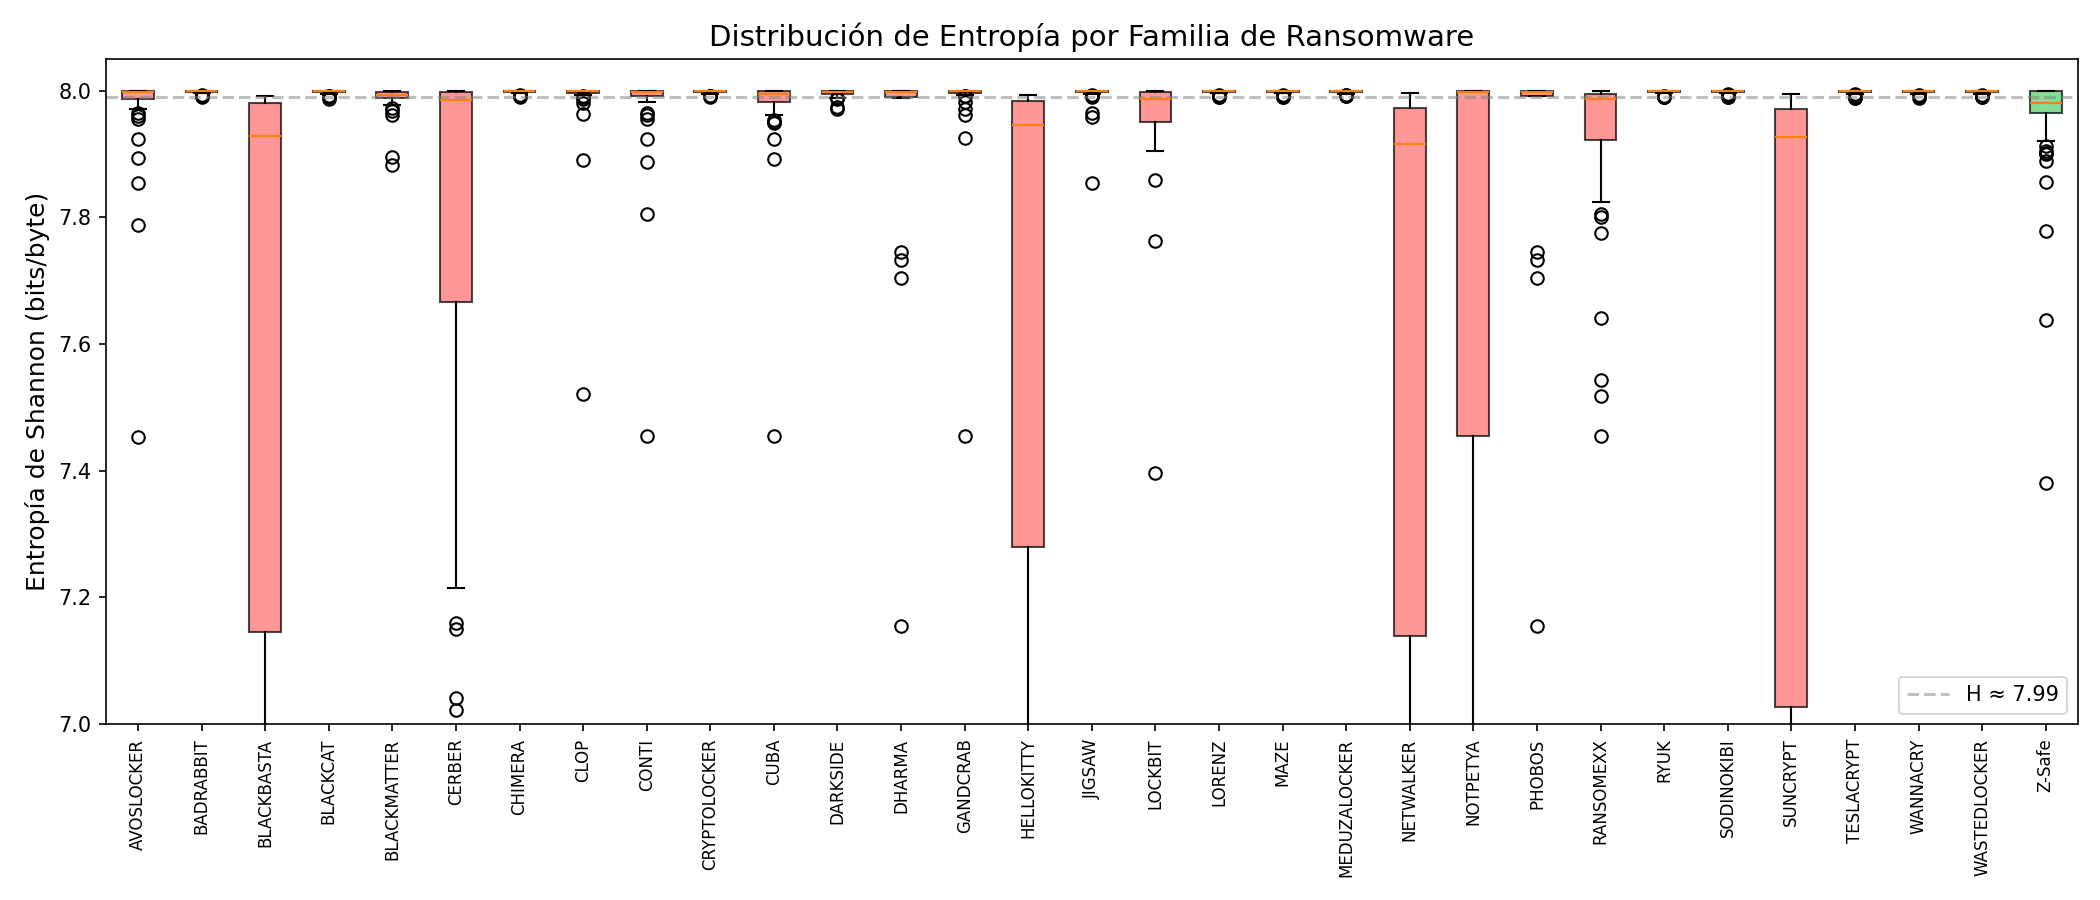
\includegraphics[width=0.95\textwidth]{images/fig_entropia_por_familia.png}
\caption{Distribución de la entropía de Shannon de los archivos cifrados por familia. La convergencia de todas las familias hacia valores próximos a 8,0 bits/byte muestra que la aleatoriedad global no discrimina.}
\label{fig:entropia_familia}
\end{figure}

Sin embargo, esta conclusión resultó ser demasiado amplia. El experimento anterior emplea únicamente dos características (entropía global y tamaño) sobre 1.600 archivos, y cabe la objeción legítima de que el resultado negativo se deba a la pobreza del espacio de representación y no a una propiedad de los datos. La Sección~\ref{subsec:exp2_ampliacion} pone a prueba esa objeción, y la respuesta obliga a reformular el hallazgo.

\subsection{Ampliación del espacio de características}
\label{subsec:exp2_ampliacion}

Para descartar que la baja exactitud fuera un artefacto de un espacio de representación insuficiente, se repitió el experimento sobre el conjunto completo de NapierOne-\textit{small}~\cite{paper_7_napierone} ---29.029 archivos, 1.001 por cada una de las 29 familias disponibles--- ampliando de 2 a \textbf{275 características} por archivo. Además de las métricas estadísticas globales ya descritas, se incorporaron: entropía calculada por regiones (cabecera, cola y bloques intermedios), desvío estándar de la entropía entre bloques, diferencia de entropía entre cabecera y cola, longitud de la racha más larga de bytes repetidos, proporción de bytes nulos y de caracteres imprimibles, número de bytes distintos, y la distribución completa de frecuencia de los 256 valores de byte posibles.

Se evaluaron cinco subconjuntos de características con tres algoritmos, mediante validación cruzada estratificada de 5 particiones. Se empleó \texttt{HistGradientBoostingClassifier} en lugar del \textit{Gradient Boosting} clásico porque, con 29 clases, este último requiere entrenar $n_{\text{clases}} \times n_{\text{estimadores}} = 2.900$ árboles por ajuste, lo que resulta computacionalmente inviable sobre 29.000 muestras; la implementación basada en histogramas es el equivalente recomendado para conjuntos con más de 10.000 muestras~\cite{sklearn}. Los resultados se presentan en la Tabla~\ref{tab:exp2_ampliado}.

\begin{table}[ht]
\centering
\caption{Exactitud multiclase (29 familias) según el subconjunto de características. Validación cruzada de 5 particiones sobre 29.029 archivos. Azar $= 0{,}034$.}
\label{tab:exp2_ampliado}
\begin{tabular}{|l|c|c|c|}
\hline
\textbf{Subconjunto de características} & \textbf{Random Forest} & \textbf{KNN-5} & \textbf{HistGB} \\
\hline
Entropía global + tamaño (2) & 0,166 & 0,126 & 0,163 \\
Estadísticas globales (9) & 0,391 & 0,300 & 0,399 \\
Frecuencia de bytes (256) & 0,184 & 0,082 & 0,199 \\
Todas las características (275) & 0,542 & 0,143 & 0,592 \\
\textbf{Estadísticas + derivadas (19)} & \textbf{0,603} & 0,299 & 0,598 \\
\hline
\end{tabular}
\end{table}

El resultado es inequívoco: con un espacio de representación adecuado la exactitud pasa de 0,166 a \textbf{0,603}, casi dieciocho veces el azar. La afirmación de que las propiedades estadísticas no permiten distinguir familias, tal como se formuló a partir del experimento inicial, es incorrecta.

Conviene precisar que estos valores se obtuvieron con la configuración por defecto de cada algoritmo, sin búsqueda de hiperparámetros. La optimización se reservó para las dos configuraciones que resultaron determinantes ---el clasificador sobre bytes (Sección~\ref{sec:exp2c}) y el clasificador de notas (Sección~\ref{subsec:exp3_hiperparametros})--- por dos motivos: el propósito de este experimento es delimitar el alcance del resultado negativo inicial, para lo cual basta demostrar que la exactitud crece sustancialmente al ampliar la representación; y el valor aquí obtenido queda superado por el del Experimento 2c sobre el mismo conjunto de datos, de modo que una optimización adicional no alteraría las conclusiones. Se señala como limitación explícita del alcance de este experimento.

Dos observaciones secundarias merecen registrarse. En primer lugar, las 275 características (0,592) rinden ligeramente \textit{peor} que 19 seleccionadas por criterio experto (0,603): las 256 frecuencias de byte introducen ruido sin aportar señal, un caso claro de maldición de la dimensionalidad. En segundo lugar, la selección automática por prueba F de ANOVA no mejora ese resultado (0,363 con 10 características, 0,387 con 50), lo que confirma que el aporte proviene de la interacción entre características y no de unas pocas individualmente dominantes.

\subsection{Dónde reside la información discriminante}
\label{subsec:exp2_donde}

El análisis de importancia de características del Random Forest~\cite{breiman2001} explica el resultado anterior y constituye, a juicio de este trabajo, el hallazgo conceptual más relevante del frente de archivos cifrados. La Tabla~\ref{tab:exp2_importancias} presenta las diez características más informativas.

\begin{table}[ht]
\centering
\caption{Características más discriminativas según la importancia de Gini del Random Forest}
\label{tab:exp2_importancias}
\begin{tabular}{|c|l|c|l|}
\hline
\textbf{\#} & \textbf{Característica} & \textbf{Importancia} & \textbf{Qué mide} \\
\hline
1 & \texttt{longest\_run} & 0,0715 & Racha más larga de bytes repetidos \\
2 & \texttt{entropy\_diff\_hf} & 0,0412 & Diferencia de entropía cabecera--cola \\
3 & \texttt{entropy\_footer} & 0,0402 & Entropía de la cola del archivo \\
4 & \texttt{entropy\_header} & 0,0314 & Entropía de la cabecera \\
5 & \texttt{chi\_square} & 0,0148 & Estadístico $\chi^2$ global \\
6 & \texttt{zero\_ratio} & 0,0111 & Proporción de bytes nulos \\
7 & \texttt{byte\_freq\_000} & 0,0108 & Frecuencia del byte \texttt{0x00} \\
8 & \texttt{file\_size} & 0,0095 & Tamaño del archivo \\
9 & \texttt{block\_entropy\_std} & 0,0081 & Variación de entropía entre bloques \\
10 & \texttt{byte\_freq\_max} & 0,0074 & Frecuencia del byte más común \\
\hline
\end{tabular}
\end{table}

Ninguna de las características dominantes mide la calidad criptográfica del cifrado. Todas miden, de una u otra forma, \textbf{la presencia de datos no aleatorios dentro de un archivo por lo demás aleatorio}: rachas de bytes repetidos, asimetría de entropía entre el comienzo y el final, exceso de bytes nulos, variación de entropía entre bloques. Son indicadores indirectos de que la familia ha añadido una cabecera, una cola o un bloque de relleno al contenido cifrado.

Esto reformula el resultado del Experimento 2 en los siguientes términos, que son los que este trabajo sostiene:

\begin{quote}
La información que permite distinguir familias de ransomware a partir de sus archivos cifrados no reside en las propiedades criptográficas del contenido ---que son, en efecto, indistinguibles--- sino en la \textbf{estructura} del archivo: en los artefactos no aleatorios que cada familia añade deliberadamente. Medida globalmente, la aleatoriedad no discrimina (0,166); medida por regiones y rachas, alcanza 0,603.
\end{quote}

Esta lectura es además coherente con la capacidad de ID Ransomware de identificar el 66,67\% de las familias a partir de archivos cifrados (Sección~\ref{sec:res_herramientas}): la herramienta no emplea estadística sino firmas de bytes en posiciones conocidas. Las dos secciones siguientes ponen a prueba esta hipótesis de forma directa, primero localizando explícitamente esas firmas (Experimento 2b) y luego aprendiéndolas de los datos (Experimento 2c).

\section{Experimento 2b: Identificación por Artefactos Estructurales}
\label{sec:exp2b}

\subsection{Motivación y diseño}

Dos observaciones independientes motivaron este experimento. La primera surgió de la evaluación de herramientas descrita en la Sección~\ref{sec:res_herramientas}: de las veinte familias que ID Ransomware~\cite{idransomware} identifica correctamente a partir de un archivo cifrado, nueve mantienen la identificación aun cuando el archivo se renombra, lo que implica necesariamente que la evidencia utilizada está en el contenido y no en el nombre. La segunda proviene de la literatura: Davies et al.~\cite{davies2023majority} incorporan una prueba de \textit{magic number} a su sistema de detección por votación mayoritaria, alcanzando 0,961 de exactitud en la tarea binaria, lo que confirma que las firmas de bytes son un indicador explotable.

Ambas fuentes utilizan, sin embargo, catálogos de firmas construidos manualmente. El experimento aquí propuesto invierte el procedimiento: en lugar de partir de una lista conocida, las firmas se \textbf{descubren automáticamente a partir de los datos}. Para cada familia se calcula el prefijo y el sufijo binario común a todos sus archivos (el mayor prefijo y sufijo comunes sobre una ventana de 64 bytes) y la extensión añadida común. Una familia se considera estructuralmente identificable si posee un prefijo o sufijo común de al menos 4 bytes, o una extensión propia.

La clasificación se evalúa mediante el procedimiento \textit{leave-one-out}: para cada archivo, las marcas de todas las familias se recalculan excluyendo ese archivo, de modo que la predicción nunca se apoya en información derivada de la muestra evaluada. Se evaluaron 1.450 archivos (50 por familia).

\subsection{Marcas descubiertas}

El procedimiento identificó marcas estructurales en \textbf{25 de las 29 familias}. En quince casos se trata de firmas binarias en el contenido, varias de ellas legibles como texto: WANNACRY escribe \texttt{57 41 4E 41 43 52 59 21} al inicio de cada archivo, secuencia que corresponde a la cadena \texttt{WANACRY!}; CUBA inserta \texttt{FIDEL.CA} en los primeros veinte bytes; PHOBOS añade \texttt{LOCK96} al final. Otras familias emplean firmas extensas no textuales: CERBER, LOCKBIT, RANSOMEXX y TESLACRYPT presentan bloques constantes de 64 bytes.

Este resultado valida de forma independiente las anotaciones manuales realizadas durante la evaluación de ID Ransomware: las nueve familias cuya identificación sobrevivía al renombrado figuran entre las que el procedimiento automático detecta con firma binaria.

Cuatro familias ---BADRABBIT, JIGSAW, NOTPETYA y SUNCRYPT--- no presentan marca alguna. El caso de NOTPETYA coincide con lo documentado por Davies et al.~\cite{davies2023majority}, quienes observan que esta familia no modifica la extensión de los archivos que ataca y que, por ese motivo, evade las pruebas basadas en nombre y extensión. La convergencia entre ambos trabajos, obtenida por vías metodológicas distintas, refuerza la validez del procedimiento.

\subsection{Resultados y ablación}

Un resultado agregado del 86,2\% de exactitud podría atribuirse por completo a la extensión del archivo, que es también el mecanismo que emplean las herramientas basadas en reglas. Para separar ambas contribuciones se repitió la evaluación en tres modalidades (Tabla~\ref{tab:exp2b}).

\begin{table}[ht]
\centering
\caption{Ablación del Experimento 2b: contribución de cada tipo de marca (1.450 archivos, 29 familias, \textit{leave-one-out})}
\label{tab:exp2b}
\begin{tabular}{|l|c|c|c|}
\hline
\textbf{Modalidad} & \textbf{Cobertura} & \textbf{Exactitud global} & \textbf{Exactitud donde aplica} \\
\hline
Solo extensión del archivo & 82,8\% & 0,828 & 1,000 \\
Solo firmas binarias & 53,3\% & 0,517 & 0,970 \\
Combinado & 87,8\% & 0,862 & 0,982 \\
\hline
\end{tabular}
\end{table}

La interpretación de estas cifras exige cautela. La extensión acierta el 100\% de los casos en que está presente, pero ese valor perfecto es un indicio de artefacto y no de mérito: en NapierOne cada familia está representada por una única campaña, de modo que su extensión es constante dentro del conjunto de datos. En la práctica, familias como DHARMA emplean extensiones que incorporan un identificador de la víctima, por lo que la extensión constituye un identificador de \textit{campaña} y no de \textit{familia}. Su rendimiento no es extrapolable.

Las firmas binarias, en cambio, constituyen evidencia de contenido: son marcadores que el propio programa escribe en el archivo para reconocer posteriormente lo que ya ha cifrado, y por lo tanto resultan más estables entre campañas que la extensión. Alcanzan un 97,0\% de acierto, pero solo cubren el 53,3\% de los archivos: la regla de coincidencia exacta exige que la firma sea idéntica en \textit{todos} los archivos de la familia, y un único caso divergente la elimina. Esta limitación de cobertura es la que motiva el experimento siguiente.

\section{Experimento 2c: Aprendizaje Automático sobre la Estructura de Bytes}
\label{sec:exp2c}

\subsection{Motivación y diseño}

El Experimento 2b localizó la información discriminante pero la explotó mediante reglas de coincidencia exacta, con la consiguiente pérdida de cobertura. Este experimento sustituye la regla por un clasificador entrenado sobre los mismos datos, con tres objetivos: alcanzar cobertura total, tolerar variabilidad parcial en las marcas, y determinar si existe información aprovechable en las familias donde la regla exacta no encontró nada.

Se extraen los \textbf{512 primeros y 512 últimos bytes} de cada archivo. De forma deliberada, \textbf{no se utiliza el nombre ni la extensión}: dado que el Experimento 2b mostró que la extensión identifica la campaña, restringir la entrada al contenido permite medir qué información reside efectivamente en los bytes.

Se compararon dos representaciones, análogas a las empleadas con las notas de rescate:

\begin{itemize}
\item \textbf{Posicional}: los 1.024 bytes como valores en posiciones fijas. Captura marcas ancladas a desplazamientos determinados. Se emplean modelos basados en árboles, que particionan por valor exacto; se descartó el uso de modelos lineales sobre esta representación porque los valores de byte son categóricos y no ordinales, de modo que la relación de orden que un modelo lineal presupone carece de sentido.
\item \textbf{N-gramas de bytes}: los mismos bytes tratados como una secuencia de símbolos, con ponderación TF-IDF de n-gramas. Captura marcas en posición variable, y constituye el análogo directo de los n-gramas de caracteres empleados en el Experimento 3.
\end{itemize}

La selección de hiperparámetros se realizó mediante búsqueda aleatorizada \textbf{anidada}: la búsqueda se ejecuta dentro del subconjunto de entrenamiento de cada partición externa, de modo que la métrica reportada no está sesgada por el proceso de selección. La búsqueda empleó una submuestra estratificada de 5.800 archivos (200 por familia) y la mejor configuración se reevaluó sobre 14.500 archivos (500 por familia) con validación cruzada de 5 particiones.

\subsection{Resultados}

\begin{table}[ht]
\centering
\caption{Experimento 2c: clasificación mediante aprendizaje sobre bytes de cabecera y cola. Cobertura del 100\% en todas las configuraciones. Sin uso de nombre ni extensión.}
\label{tab:exp2c}
\begin{tabular}{|l|c|c|c|}
\hline
\textbf{Configuración} & \textbf{Archivos} & \textbf{Exactitud} & \textbf{Macro-F1} \\
\hline
Posicional + Random Forest (búsqueda) & 5.800 & 0,897 & 0,897 \\
N-gramas de bytes + Regresión Logística & 5.800 & 0,856 & 0,858 \\
N-gramas de bytes + LinearSVC & 5.800 & 0,849 & 0,846 \\
\hline
\textbf{Posicional + Random Forest (final)} & \textbf{14.500} & \textbf{0,910} & \textbf{0,908} \\
\hline
\end{tabular}
\end{table}

La mejor configuración alcanza una \textbf{exactitud de 0,910 y un macro-F1 de 0,908 sobre 29 familias, con cobertura total y utilizando exclusivamente el contenido del archivo}. Los hiperparámetros seleccionados fueron 300 árboles, profundidad máxima 20, mínimo de 2 muestras por hoja y 30\% de características por división.

Resulta significativo que la representación posicional supere a los n-gramas de bytes: las marcas se encuentran en \textbf{desplazamientos fijos} del archivo, coherente con cabeceras y colas escritas por el programa en posiciones determinísticas. Este comportamiento contrasta con el observado en las notas de rescate, donde los n-gramas de caracteres resultan la mejor representación; la diferencia refleja la naturaleza distinta de ambos artefactos, uno generado por código y el otro redactado por personas.

\subsection{Análisis por familia}

La Figura~\ref{fig:f1_bytes} presenta el F1 obtenido por cada familia, distinguiendo qué tipo de marca había detectado el Experimento 2b.

\begin{figure}[ht]
\centering
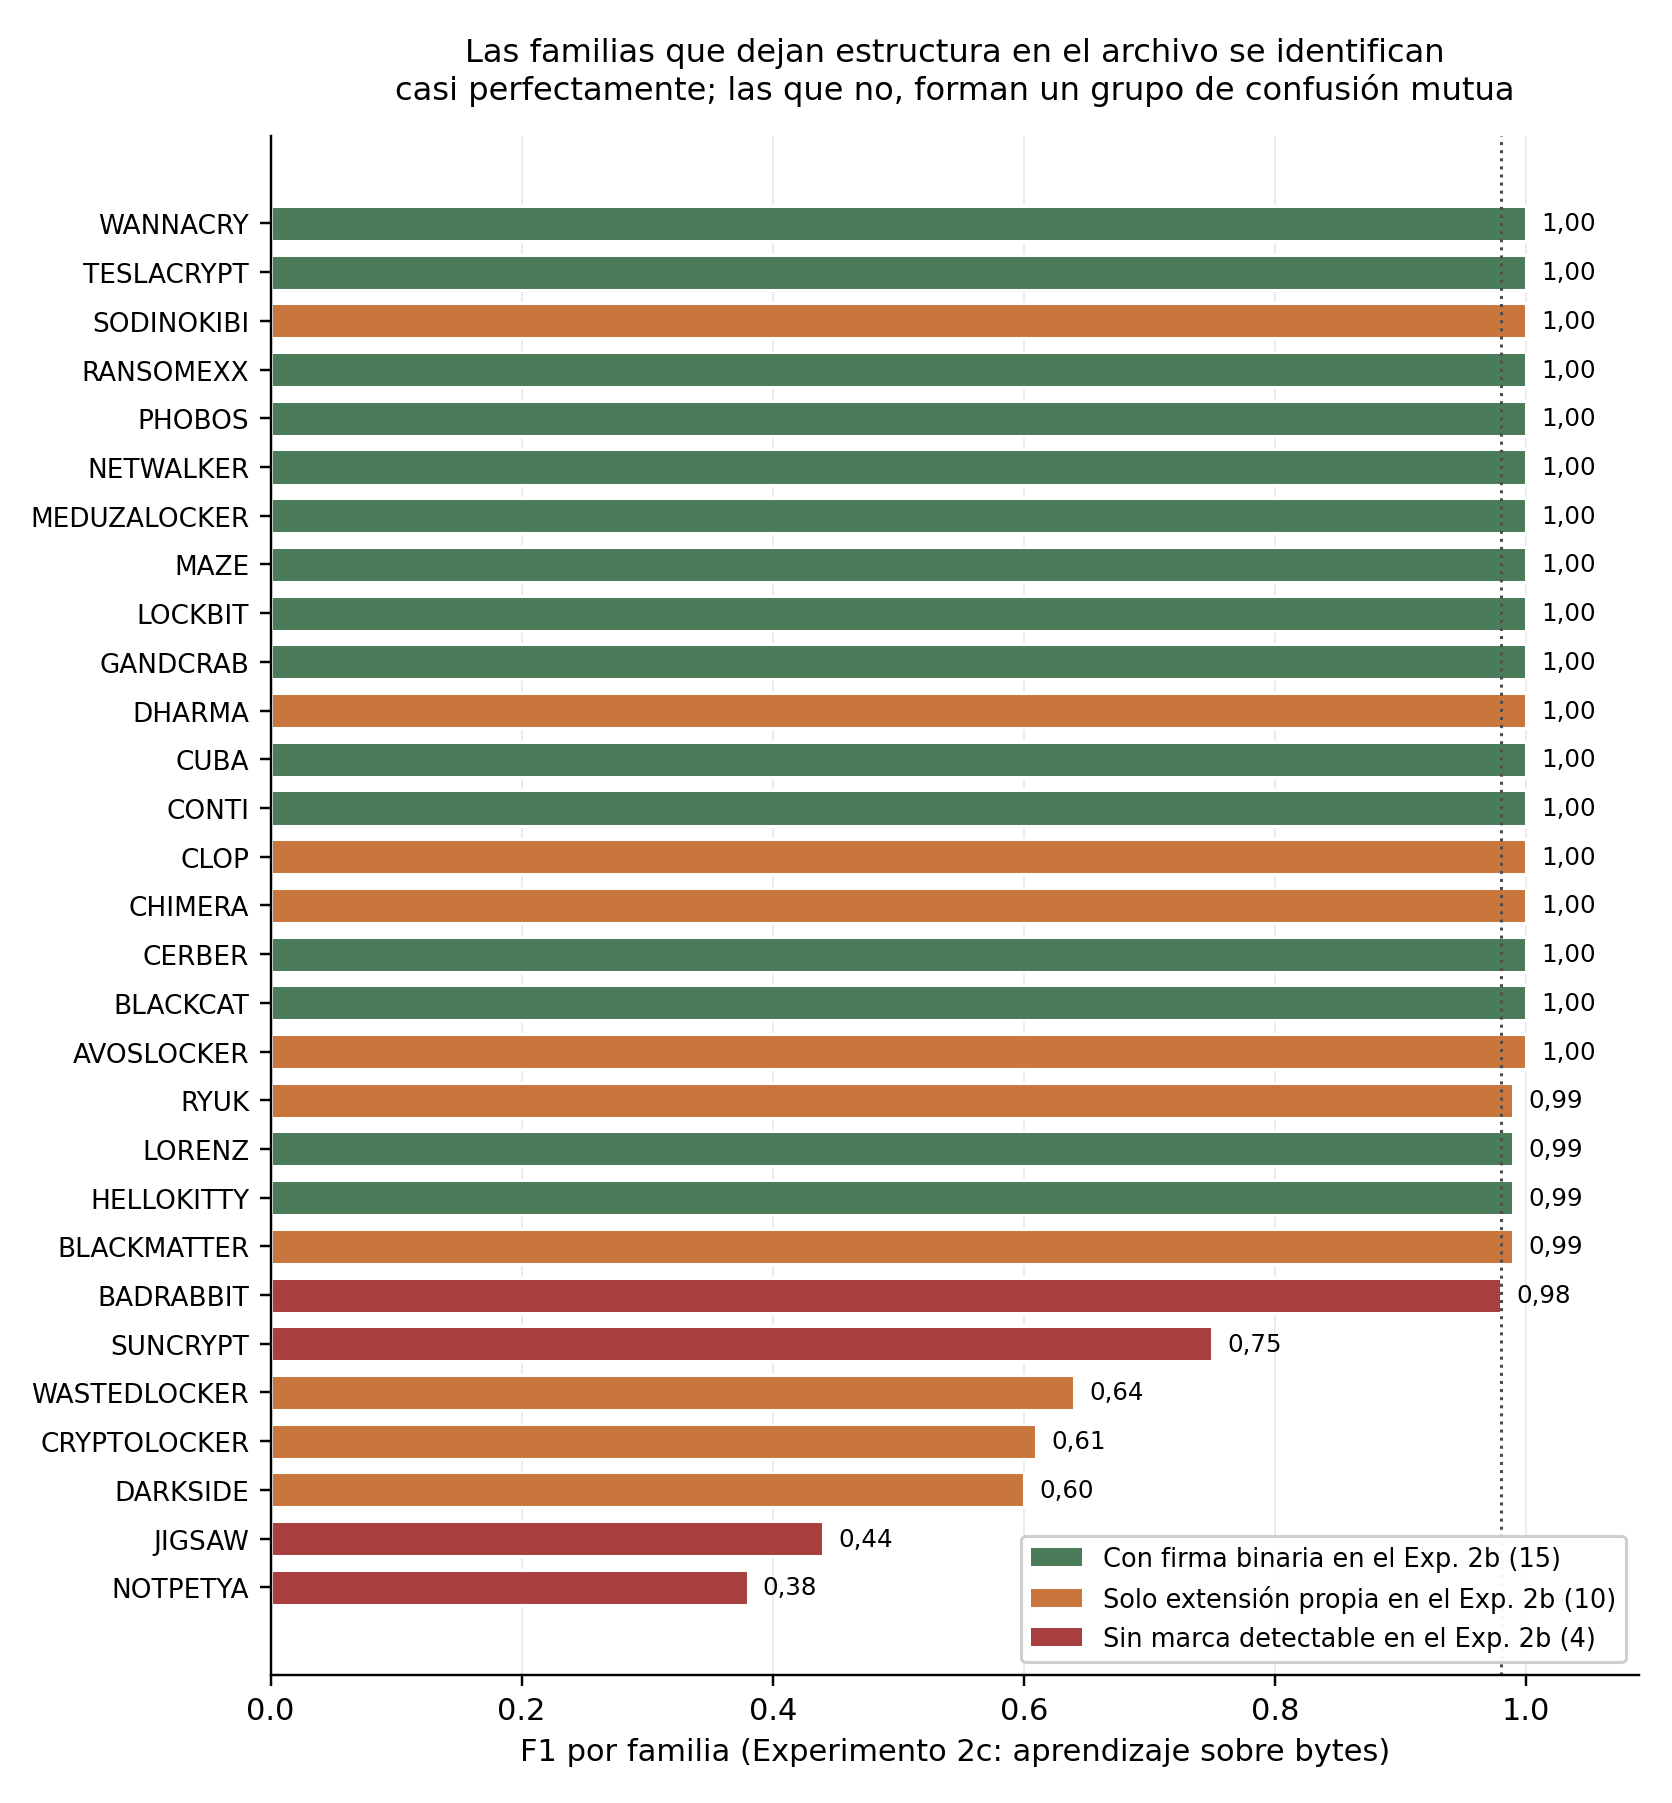
\includegraphics[width=0.86\textwidth]{images/fig_f1_por_familia_bytes.png}
\caption{F1 por familia en el Experimento 2c. El color indica el tipo de marca detectada por el Experimento 2b. Las quince familias con firma binaria se identifican sin excepción por encima de 0,99; siete de las diez que solo poseían extensión propia también, lo que indica que el clasificador halla patrones de contenido que la regla de coincidencia exacta no detecta.}
\label{fig:f1_bytes}
\end{figure}

El resultado es marcadamente bimodal: \textbf{23 de las 29 familias alcanzan un F1 igual o superior a 0,98}, mientras que seis quedan por debajo de 0,76. La correspondencia con el Experimento 2b es notable y opera como validación cruzada entre ambos:

\begin{itemize}
\item Las \textbf{quince familias con firma binaria} identificada en el Experimento 2b obtienen, sin una sola excepción, un F1 igual o superior a 0,99.
\item De las \textbf{diez familias que solo poseían extensión propia} ---es decir, sin marca detectable en el contenido mediante coincidencia exacta---, siete alcanzan igualmente valores superiores a 0,99. El clasificador extrae de los bytes información que la regla exacta no capturaba.
\item De las \textbf{cuatro familias sin marca alguna}, BADRABBIT pasa de un F1 de 0,15 en el experimento estadístico a \textbf{0,98}, quedando plenamente resuelta. SUNCRYPT (0,75), NOTPETYA (0,38) y JIGSAW (0,44) mejoran respecto de los experimentos previos pero permanecen entre las difíciles.
\end{itemize}

Las seis familias con menor rendimiento ---SUNCRYPT (0,75), WASTEDLOCKER (0,64), CRYPTOLOCKER (0,61), DARKSIDE (0,60), JIGSAW (0,44) y NOTPETYA (0,38)--- forman un grupo de confusión mutua. DARKSIDE presenta un patrón revelador: precisión de 0,45 frente a un recall de 0,90, lo que indica que actúa como clase de destino por defecto para los archivos que el modelo no logra atribuir. Estas seis familias son, presumiblemente, las que cifran sin añadir estructura al archivo, y constituyen el residuo genuino de la indistinguibilidad estadística planteada en el Experimento 2.

\subsection{Limitación}
\label{subsec:exp2c_limitacion}

El conjunto NapierOne representa cada familia mediante una única campaña, obtenida ejecutando una muestra concreta del ransomware. En consecuencia, el valor de 0,910 mide la capacidad de identificar \textit{esa campaña}, y no puede afirmarse que se extienda a campañas futuras de la misma familia, que podrían modificar sus cabeceras o colas. Esta limitación es análoga a la observada en el corpus de notas de rescate, donde la baja variabilidad de plantillas produce el mismo efecto (Sección~\ref{subsec:res_variabilidad}), y su evaluación requeriría un conjunto de datos con múltiples campañas por familia, no disponible en la actualidad.

\section{Síntesis del Frente de Archivos Cifrados}
\label{sec:sintesis_archivos}

La Figura~\ref{fig:progresion} resume la progresión de los cuatro enfoques evaluados sobre el mismo conjunto de archivos cifrados.

\begin{figure}[ht]
\centering
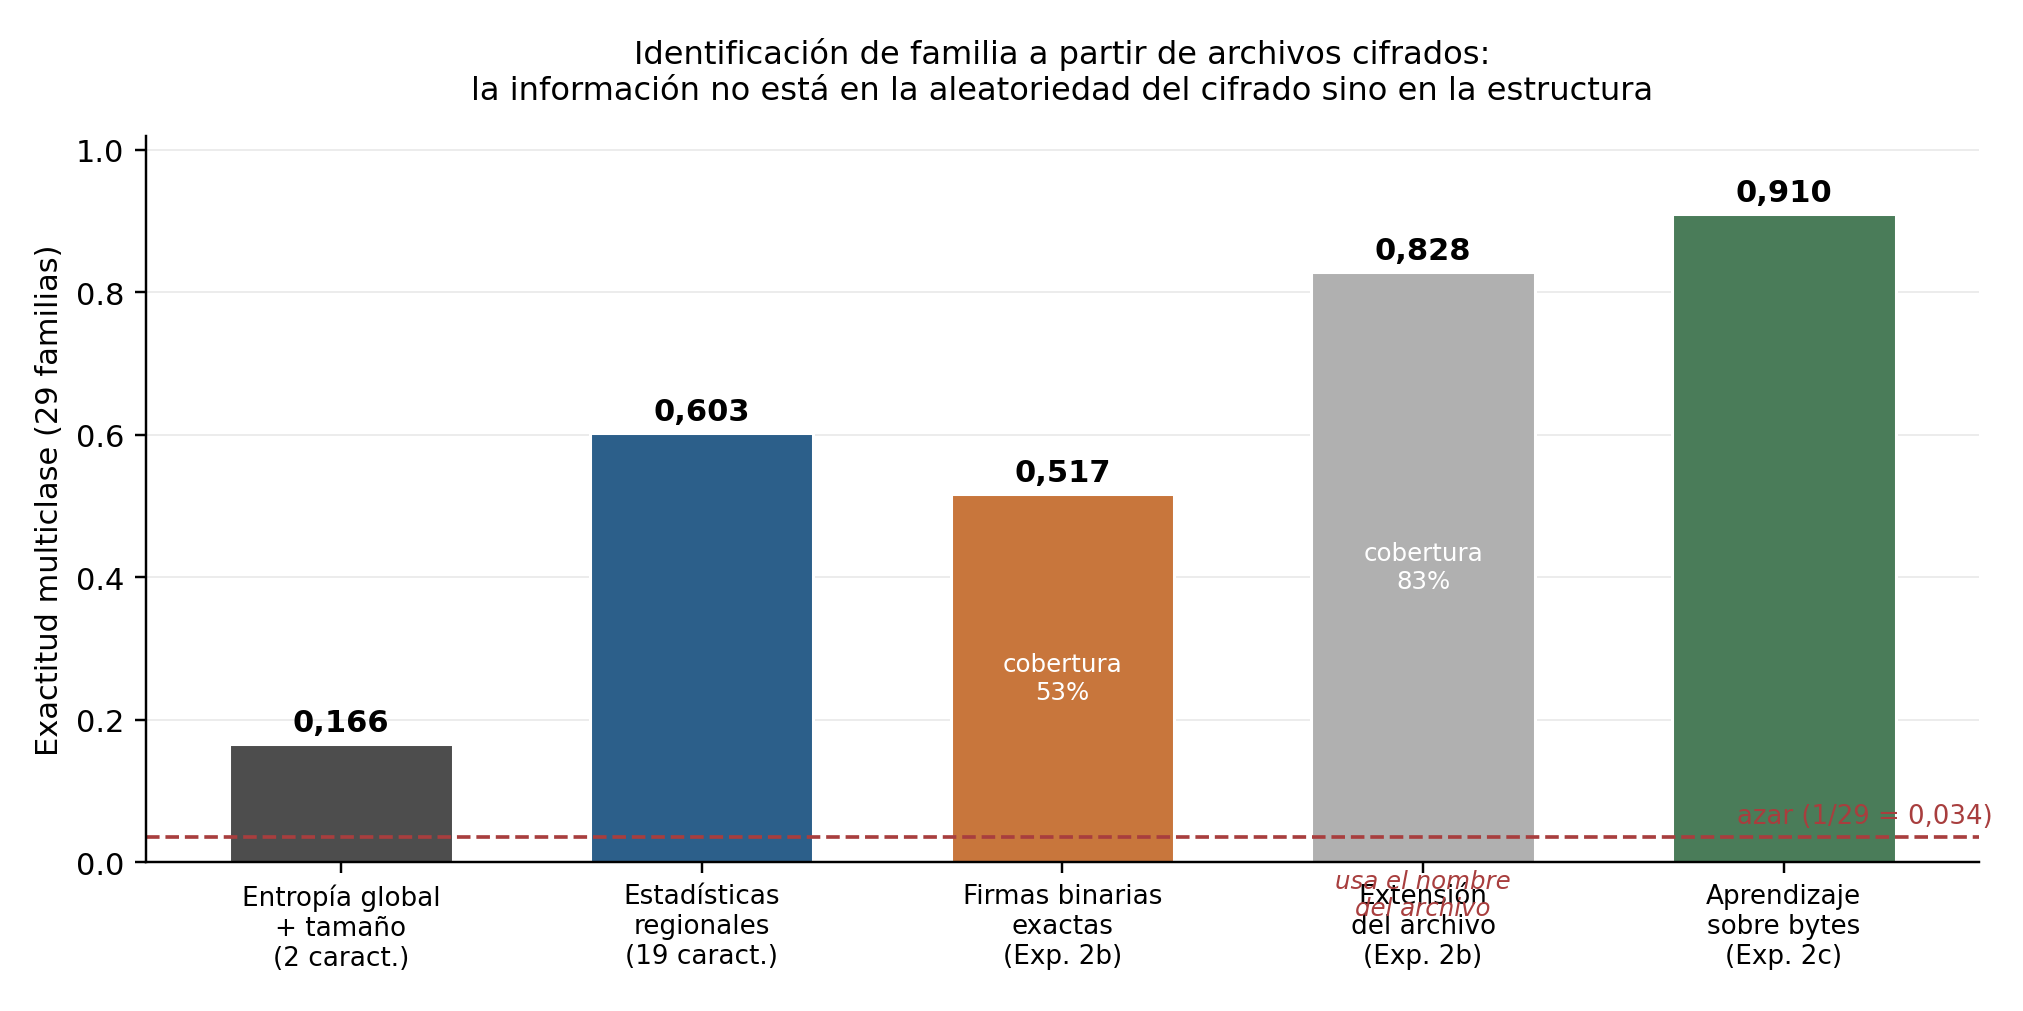
\includegraphics[width=0.95\textwidth]{images/fig_progresion_archivos.png}
\caption{Progresión de enfoques para la identificación de familia a partir de archivos cifrados. Cada enfoque responde a una limitación del anterior. El valor de la extensión se muestra en gris por tratarse de un identificador de campaña.}
\label{fig:progresion}
\end{figure}

Cada etapa responde a una objeción de la anterior: la ampliación del espacio de características descarta que el resultado negativo inicial se debiera a una representación pobre; la localización explícita de firmas identifica dónde reside la señal; y el aprendizaje sobre bytes extiende esa señal a la totalidad del conjunto sin recurrir a metadatos del nombre.

La conclusión del frente de archivos cifrados queda, por tanto, acotada con precisión: la indistinguibilidad estadística es real, pero se limita a \textbf{seis de las veintinueve familias evaluadas}, aquellas que cifran sin dejar estructura reconocible. Para las veintitrés restantes la información de familia está presente en el contenido del archivo y es extraíble automáticamente con una exactitud del 0,910.

\section{Experimento 3: Clasificación por Notas de Rescate (NLP)}
\label{sec:exp3}

\subsection{Variabilidad del Corpus: las Notas como Plantillas}
\label{subsec:res_variabilidad}

El análisis de casi-duplicados (Sección~\ref{subsec:neardups}) revela un fenómeno central para interpretar los resultados: \textbf{las 146 notas del corpus contienen solo 95 grupos de contenido distinto}. Las notas de rescate son plantillas que cada familia reutiliza modificando únicamente datos de contacto o identificadores de víctima. Los casos extremos son ilustrativos: las 19 notas de DHARMA corresponden a solo 6 plantillas (el mismo texto con distinta dirección de correo), las 18 de CERBER a 8, y las 4 de WASTEDLOCKER a una única plantilla.

Esta baja variabilidad intra-familia tiene dos consecuencias metodológicas: fundamenta el uso de los dos protocolos de evaluación (P1 y P2), y demuestra que la expansión del corpus debe medirse en \textit{plantillas} nuevas por familia, no solo en cantidad de archivos.

\subsection{Resultados bajo el Protocolo P1 (plantilla conocida)}

La Tabla~\ref{tab:exp3_p1} presenta los resultados del protocolo P1, que mide la capacidad de identificar la familia de una nueva instancia de una plantilla ya catalogada.

\begin{table}[ht]
\centering
\caption{Clasificación NLP bajo el protocolo P1 (146 notas, 30 familias, 2-fold CV $\times$ 10 semillas)}
\label{tab:exp3_p1}
\resizebox{\textwidth}{!}{
\begin{tabular}{|l|l|c|c|c|c|}
\hline
\textbf{TF-IDF} & \textbf{Modelo} & \textbf{Accuracy} & \textbf{Balanced acc.} & \textbf{Macro-F1} & \textbf{Weighted-F1} \\
\hline
\multirow{4}{*}{Palabras (1-2)} & LinearSVC & 0,821 & 0,770 & 0,748 $\pm$ 0,032 & 0,799 \\
 & Reg. Logística & 0,790 & 0,759 & 0,728 $\pm$ 0,029 & 0,770 \\
 & Random Forest & 0,749 & 0,664 & 0,660 $\pm$ 0,034 & 0,717 \\
 & KNN & 0,678 & 0,535 & 0,488 $\pm$ 0,032 & 0,632 \\
\hline
\multirow{4}{*}{Caracteres (3-5)} & LinearSVC & 0,818 & \textbf{0,777} & \textbf{0,760 $\pm$ 0,029} & 0,798 \\
 & Reg. Logística & 0,791 & 0,763 & 0,733 $\pm$ 0,035 & 0,769 \\
 & Random Forest & 0,745 & 0,645 & 0,626 $\pm$ 0,036 & 0,707 \\
 & KNN & 0,671 & 0,523 & 0,481 $\pm$ 0,025 & 0,626 \\
\hline
\multirow{4}{*}{Combinado} & LinearSVC & \textbf{0,825} & 0,769 & 0,754 $\pm$ 0,033 & \textbf{0,804} \\
 & Reg. Logística & 0,803 & 0,760 & 0,739 $\pm$ 0,031 & 0,782 \\
 & Random Forest & 0,753 & 0,660 & 0,647 $\pm$ 0,025 & 0,719 \\
 & KNN & 0,691 & 0,542 & 0,503 $\pm$ 0,026 & 0,647 \\
\hline
\end{tabular}
}
\end{table}

La mejor configuración por macro-F1 fue LinearSVC con n-gramas de caracteres (3-5): \textbf{macro-F1 de 0,760, balanced accuracy de 0,777 y accuracy de 0,818} sobre 30 clases, donde el azar equivale a 0,033. Los modelos lineales superan consistentemente a Random Forest y KNN, en línea con la efectividad conocida de los clasificadores lineales en espacios TF-IDF de alta dimensionalidad con pocas muestras~\cite{joachims1998}.

\subsection{Resultados bajo el Protocolo P2 (variante nunca vista)}

La Tabla~\ref{tab:exp3_p2} presenta los resultados del protocolo P2, en el que ninguna variante casi idéntica de una nota de prueba estuvo disponible durante el entrenamiento.

\begin{table}[ht]
\centering
\caption{Clasificación NLP bajo el protocolo P2 (grupos de casi-duplicados no repartidos, 2-fold CV $\times$ 10 semillas)}
\label{tab:exp3_p2}
\resizebox{\textwidth}{!}{
\begin{tabular}{|l|l|c|c|c|c|}
\hline
\textbf{TF-IDF} & \textbf{Modelo} & \textbf{Accuracy} & \textbf{Balanced acc.} & \textbf{Macro-F1} & \textbf{Weighted-F1} \\
\hline
\multirow{4}{*}{Palabras (1-2)} & LinearSVC & 0,535 & 0,481 & 0,422 $\pm$ 0,055 & 0,497 \\
 & Reg. Logística & 0,520 & 0,475 & 0,412 $\pm$ 0,050 & 0,479 \\
 & Random Forest & 0,486 & 0,393 & 0,363 $\pm$ 0,048 & 0,449 \\
 & KNN & 0,408 & 0,289 & 0,259 $\pm$ 0,026 & 0,374 \\
\hline
\multirow{4}{*}{Caracteres (3-5)} & LinearSVC & 0,529 & 0,470 & 0,412 $\pm$ 0,041 & 0,490 \\
 & Reg. Logística & 0,523 & 0,467 & 0,401 $\pm$ 0,048 & 0,483 \\
 & Random Forest & 0,484 & 0,383 & 0,348 $\pm$ 0,043 & 0,442 \\
 & KNN & 0,413 & 0,293 & 0,262 $\pm$ 0,036 & 0,384 \\
\hline
\multirow{4}{*}{Combinado} & LinearSVC & \textbf{0,551} & \textbf{0,492} & \textbf{0,435 $\pm$ 0,057} & \textbf{0,512} \\
 & Reg. Logística & 0,526 & 0,473 & 0,417 $\pm$ 0,051 & 0,488 \\
 & Random Forest & 0,497 & 0,397 & 0,364 $\pm$ 0,052 & 0,454 \\
 & KNN & 0,418 & 0,296 & 0,274 $\pm$ 0,045 & 0,392 \\
\hline
\end{tabular}
}
\end{table}

La mejor configuración fue la representación combinada con LinearSVC: \textbf{macro-F1 de 0,435 y accuracy de 0,551}. La caída respecto de P1 (de 0,760 a 0,435 en macro-F1) cuantifica exactamente cuánto del rendimiento aparente proviene de reconocer plantillas ya vistas: es una consecuencia directa de la baja variabilidad documentada en la Sección~\ref{subsec:res_variabilidad}, no un defecto del clasificador. Bajo P2 la representación combinada (palabras + caracteres) sí aporta una mejora sobre caracteres solos, lo que sugiere que ante variantes nuevas la información semántica y la morfológica se complementan.

\subsection{Análisis por Familia}

La Tabla~\ref{tab:exp3_familia} presenta el F1 por familia de la mejor configuración bajo P2, junto con el número de notas y de grupos de contenido distinto, y la Figura~\ref{fig:confusion_canonica} la matriz de confusión correspondiente.

\begin{table}[ht]
\centering
\caption{F1 por familia bajo P2 (combinado + LinearSVC, promedio de 10 semillas), ordenado descendentemente}
\label{tab:exp3_familia}
\resizebox{\textwidth}{!}{
\begin{tabular}{|l|c|c|c||l|c|c|c|}
\hline
\textbf{Familia} & \textbf{Notas} & \textbf{Grupos} & \textbf{F1} & \textbf{Familia} & \textbf{Notas} & \textbf{Grupos} & \textbf{F1} \\ \hline
AVOSLOCKER & 3 & 3 & 0,861 & SUNCRYPT & 2 & 2 & 0,500 \\ \hline
CERBER & 18 & 8 & 0,831 & DHARMA & 19 & 6 & 0,483 \\ \hline
GANDCRAB & 9 & 5 & 0,831 & LOCKBIT & 8 & 6 & 0,450 \\ \hline
CONTI & 4 & 3 & 0,786 & SODINOKIBI & 3 & 3 & 0,449 \\ \hline
BLACKCAT & 4 & 4 & 0,767 & CLOP & 4 & 4 & 0,378 \\ \hline
TESLACRYPT & 9 & 4 & 0,717 & BADRABBIT & 2 & 2 & 0,270 \\ \hline
LORENZ & 3 & 3 & 0,685 & HELLOKITTY & 5 & 5 & 0,248 \\ \hline
RANSOMEXX & 5 & 4 & 0,658 & CRYPTOLOCKER & 4 & 3 & 0,234 \\ \hline
BLACKMATTER & 2 & 2 & 0,650 & JIGSAW & 2 & 2 & 0,230 \\ \hline
PHOBOS & 4 & 4 & 0,637 & BLACKBASTA & 5 & 4 & 0,215 \\ \hline
DARKSIDE & 3 & 2 & 0,603 & NOTPETYA & 2 & 2 & 0,197 \\ \hline
CUBA & 4 & 2 & 0,589 & RYUK & 4 & 2 & 0,075 \\ \hline
NETWALKER & 3 & 2 & 0,586 & CHIMERA & 2 & 2 & 0,067 \\ \hline
 & & & & MEDUZALOCKER & 4 & 3 & 0,065 \\ \hline
 & & & & WANNACRY & 2 & 2 & 0,000 \\ \hline
 & & & & MAZE & 3 & 2 & 0,000 \\ \hline
 & & & & WASTEDLOCKER & 4 & 1 & 0,000 \\ \hline
\end{tabular}
}
\end{table}

\begin{figure}[ht]
\centering
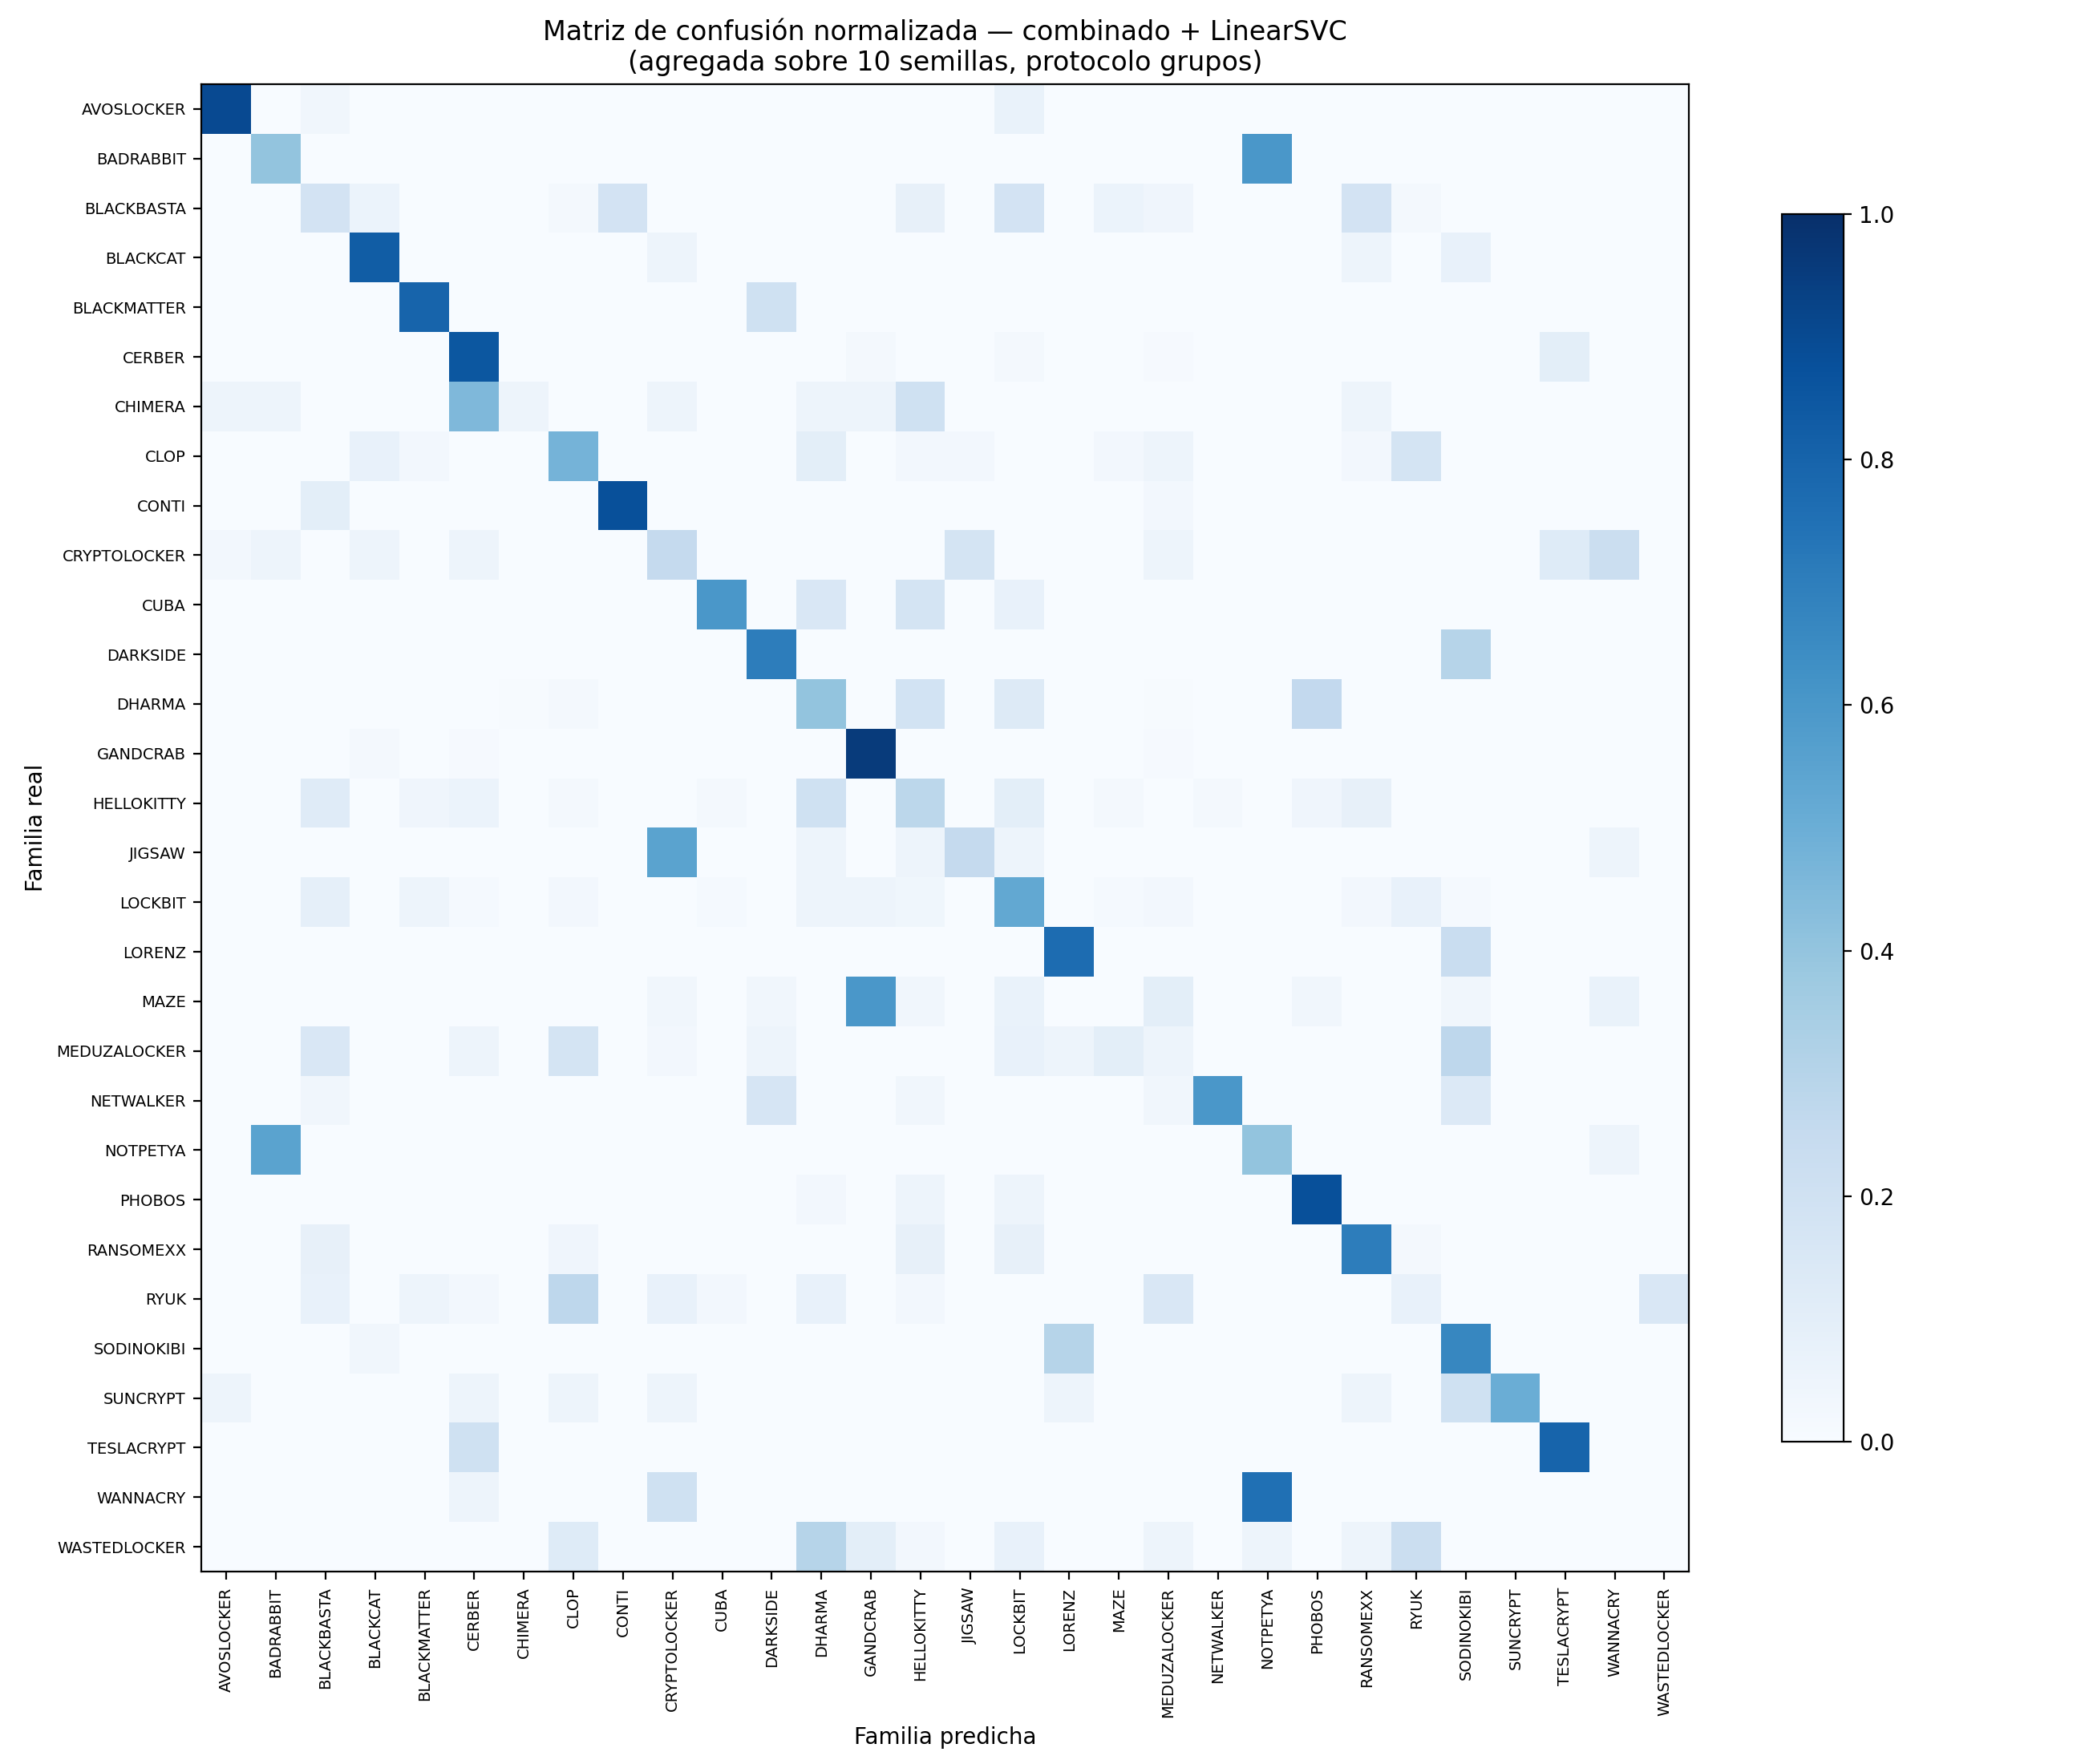
\includegraphics[width=0.95\textwidth]{images/fig_confusion_canonica.png}
\caption{Matriz de confusión normalizada de la mejor configuración bajo P2 (combinado + LinearSVC), agregada sobre las 10 repeticiones.}
\label{fig:confusion_canonica}
\end{figure}

Se observa un patrón claro: las familias con mayor diversidad de plantillas y notas extensas y distintivas (AVOSLOCKER, CERBER, GANDCRAB, CONTI, BLACKCAT) se clasifican bien incluso ante variantes nuevas, mientras que las familias con pocas plantillas o notas muy breves y genéricas (WANNACRY, MAZE, CHIMERA, RYUK) no logran generalizarse. WASTEDLOCKER constituye el caso límite: sus 4 notas forman un único grupo de contenido, por lo que bajo P2 es estructuralmente inevaluable (F1 = 0 por construcción, declarado en la Sección~\ref{subsec:protocolos_nlp}).

Este patrón converge con las observaciones de Lemmou et al.~\cite{paper_5_note_files}, cuyos falsos positivos de similitud de contenido corresponden precisamente a confusiones entre familias emparentadas (CryptoLocker con TeslaCrypt, entre otras): la dificultad de atribuir familia ante contenido nuevo o compartido es una propiedad del dominio, no un defecto del método.

\subsection{Optimización de hiperparámetros}
\label{subsec:exp3_hiperparametros}

Los resultados anteriores se obtuvieron con la configuración por defecto de cada modelo. Para descartar que el rendimiento estuviera limitado por una elección subóptima de parámetros ---objeción habitual ante un resultado que no alcanza los valores deseados--- se realizó una búsqueda sistemática sobre 360 configuraciones para la representación de palabras y 480 para la de caracteres, variando el rango de n-gramas, el tamaño máximo del vocabulario, los umbrales de frecuencia documental y el parámetro de regularización $C$.

La búsqueda se implementó de forma \textbf{anidada}: para cada partición externa, la selección de hiperparámetros se realiza mediante validación cruzada interna sobre el subconjunto de entrenamiento, y la evaluación se efectúa sobre la partición externa, que no participó de la selección. Este diseño evita el sesgo optimista que introduce elegir la configuración observando el mismo conjunto sobre el que después se reporta el resultado. El procedimiento se repitió con las diez semillas y bajo ambos protocolos.

\begin{table}[ht]
\centering
\caption{Clasificación de notas con hiperparámetros optimizados (búsqueda anidada, 144 notas, 10 semillas)}
\label{tab:exp3_hiperparametros}
\begin{tabular}{|l|c|c|}
\hline
\textbf{Configuración} & \textbf{P1 (plantilla conocida)} & \textbf{P2 (variante nueva)} \\
\hline
Palabras + LinearSVC & 0,754 $\pm$ 0,029 & 0,408 $\pm$ 0,052 \\
Palabras + Reg. Logística & 0,734 $\pm$ 0,030 & 0,400 $\pm$ 0,054 \\
Caracteres + LinearSVC & 0,742 $\pm$ 0,050 & 0,416 $\pm$ 0,060 \\
Caracteres + Reg. Logística & 0,737 $\pm$ 0,039 & 0,407 $\pm$ 0,065 \\
\textbf{Combinado, mejores hiperparámetros} & \textbf{0,775 $\pm$ 0,032} & \textbf{0,424 $\pm$ 0,064} \\
\hline
\end{tabular}
\end{table}

\textbf{La optimización no produce una mejora significativa.} Los valores obtenidos (macro-F1 de 0,775 bajo P1 y 0,424 bajo P2) son estadísticamente indistinguibles de los alcanzados con la configuración por defecto, dado que las diferencias caen dentro del desvío estándar entre semillas.

Este resultado negativo es informativo. Indica, en primer lugar, que la configuración adoptada inicialmente ---n-gramas de caracteres de 3 a 5 con LinearSVC, siguiendo la práctica establecida para clasificación de texto en espacios de alta dimensionalidad y datos dispersos~\cite{joachims1998}--- era ya adecuada para el problema. Y señala, en segundo lugar, que \textbf{el factor limitante no es la parametrización del modelo sino la composición del corpus}: con 95 plantillas distintas repartidas entre 30 familias, y siete de ellas representadas por una sola plantilla, ningún ajuste de hiperparámetros puede suplir la ausencia de ejemplos. La ampliación del corpus en profundidad queda así respaldada cuantitativamente, y no como mera recomendación.

\subsection{Comparación con los Resultados Previos del Proyecto}
\label{subsec:res_escalera}

En etapas anteriores del trabajo se reportó una accuracy del 89,7\% (macro-F1 0,840) sobre el corpus original de 156 notas. La Tabla~\ref{tab:escalera} desglosa la transición hacia los valores canónicos, en aras de la transparencia metodológica.

\begin{table}[ht]
\centering
\caption{Evolución de los resultados del Experimento 3 al corregir el protocolo de evaluación}
\label{tab:escalera}
\resizebox{\textwidth}{!}{
\begin{tabular}{|l|c|c|l|}
\hline
\textbf{Corrida} & \textbf{Accuracy} & \textbf{Macro-F1} & \textbf{Factores corregidos} \\
\hline
Corpus original (156 notas) & 0,897 & 0,840 & --- (24\% de notas duplicadas; fuga de vocabulario; \\
 & & & codificación UTF-16 mal leída; 1 semilla) \\
\hline
Canónica, protocolo P1 & 0,818 & 0,760 & deduplicación, codificación, \textit{pipeline} sin fuga, \\
 & & & 10 semillas \\
\hline
Canónica, protocolo P2 & 0,551 & 0,435 & + plantillas casi idénticas nunca repartidas \\
 & & & entre entrenamiento y prueba \\
\hline
\end{tabular}
}
\end{table}

Cada corrección reduce el valor nominal pero aumenta la validez: el 0,897 original medía en parte la capacidad del modelo de reconocer notas duplicadas; el protocolo P1 mide el reconocimiento de nuevas instancias de plantillas conocidas; y el protocolo P2, la generalización a contenido nunca visto.

\section{Ajustes al Protocolo Experimental}
\label{sec:ajustes_protocolo}

El diseño experimental presentado no se alcanzó de una sola vez. Durante la ejecución del trabajo se detectaron y corrigieron varios problemas que alteraban los resultados, y se documentan aquí por dos razones: porque las cifras previas a cada corrección circularon en informes de avance del proyecto, y porque varios de estos problemas son errores frecuentes cuya descripción puede resultar útil a trabajos similares.

\subsection{Detección de la codificación de las notas}

Catorce de las notas del corpus, pertenecientes a las familias DHARMA, GANDCRAB y SUNCRYPT, no están codificadas en UTF-8 sino en UTF-16 o cp1252. Las notas de rescate se generan en los equipos comprometidos, donde el editor predeterminado del sistema puede emplear codificaciones distintas, de modo que esta heterogeneidad es un rasgo del artefacto y no un defecto de la recolección.

La lectura de un archivo UTF-16 asumiendo UTF-8 no produce error: genera texto con bytes nulos intercalados entre los caracteres. El efecto fue doble y de signo contrario. Por un lado, trece notas ---el 8,9\% del corpus--- ingresaban al vectorizador de palabras como documentos vacíos. Por otro, en la representación de caracteres esos bytes nulos constituían una secuencia exclusiva de DHARMA y GANDCRAB, es decir, una firma sintética que el clasificador aprendía como si fuera un rasgo de esas familias. El procedimiento de lectura se modificó para detectar la codificación real de cada archivo (marca de orden de bytes, heurística de proporción de bytes nulos y retroceso a cp1252), tras lo cual ninguna nota ingresa vacía.

\subsection{Control de duplicados y casi-duplicados}

El corpus original contenía 156 notas correspondientes a 118 textos únicos: un 24\% de redundancia originada en que varias fuentes publican las mismas notas. Con una partición aleatoria, copias idénticas quedaban simultáneamente en entrenamiento y prueba, de modo que el clasificador era evaluado sobre documentos que ya había visto. La reconstrucción del corpus (\texttt{corpus\_v2}) eliminó los duplicados exactos, pero el análisis de similitud reveló que persistían pares casi idénticos ---variantes de una misma nota con distinta dirección de contacto---, lo que motivó el agrupamiento descrito en la Sección~\ref{subsec:neardups} y la adopción del protocolo P2.

\subsection{Fuga de información en la vectorización}

En la implementación inicial, el vectorizador TF-IDF se ajustaba sobre la totalidad del corpus antes de iniciar la validación cruzada. En consecuencia, el vocabulario y las frecuencias documentales inversas incorporaban información de los documentos de prueba. La corrección consistió en encapsular vectorizador y clasificador en un \texttt{Pipeline}~\cite{sklearn}, de modo que ambos se ajusten exclusivamente con el subconjunto de entrenamiento de cada partición, replicando la situación real de aplicación sobre una nota no vista previamente.

\subsection{Estabilidad de la estimación}

Con 144 documentos repartidos en 30 clases, una única partición aleatoria puede producir estimaciones no representativas. La validación se repite con diez semillas distintas y se reporta la media junto con el desvío estándar entre repeticiones, lo que permite además distinguir diferencias reales entre configuraciones de la variabilidad propia del muestreo, como fue el caso en el análisis de hiperparámetros (Sección~\ref{subsec:exp3_hiperparametros}).

\subsection{Selección de métricas}

Los informes iniciales del proyecto reportaban un 87,58\% que correspondía a la exactitud global, acompañada de métricas promediadas de forma ponderada por el tamaño de cada clase. Dado que las dos familias más numerosas concentran el 25\% del corpus, ese promedio queda dominado por ellas y sobreestima el rendimiento sobre las familias pequeñas, que son precisamente las de mayor interés operativo. Se adoptó en consecuencia el macro-F1 como métrica principal, acompañado de la exactitud balanceada, el informe por familia y la matriz de confusión. La diferencia entre ambos promedios ---0,798 ponderado frente a 0,760 macro bajo el protocolo P1--- cuantifica el sesgo.

\subsection{Ejecución en infraestructura compartida}

Los experimentos sobre el conjunto completo de NapierOne se ejecutaron en el clúster computacional del NIDTEC, gestionado mediante SLURM. Tres trabajos fueron cancelados por el sistema antes de completarse, por causas relacionadas entre sí que se documentan por su valor práctico: la asignación de memoria por defecto (2 GB) resulta insuficiente y debe solicitarse de forma explícita; la configuración \texttt{n\_jobs=-1}, habitual en un equipo personal, reserva la totalidad de los núcleos del nodo en lugar de los asignados al trabajo, por lo que se sustituyó por la lectura de la variable de entorno correspondiente; y la combinación de paralelismo en la validación cruzada con paralelismo interno del modelo generaba una multiplicación de procesos, cada uno con su propia copia de la matriz de características. Corregidos estos aspectos, la extracción de características sobre 29.029 archivos requirió 5,5 horas y el entrenamiento posterior 20 minutos.

\section{Evaluación de Herramientas Existentes}
\label{sec:res_herramientas}

La Tabla~\ref{tab:herramientas} resume la evaluación experimental de CryptoSheriff~\cite{cryptosheriff} e ID Ransomware~\cite{idransomware} descrita en la Sección~\ref{sec:met_herramientas}.

\begin{table}[ht]
\centering
\caption{Evaluación experimental de herramientas públicas de identificación de ransomware}
\label{tab:herramientas}
\begin{tabular}{|l|l|c|}
\hline
\textbf{Herramienta} & \textbf{Entrada} & \textbf{Identificación correcta} \\
\hline
CryptoSheriff & Archivos cifrados (30 familias) & 5/30 (16,67\%) \\
ID Ransomware & Archivos cifrados (30 familias) & 20/30 (66,67\%) \\
ID Ransomware & Notas de rescate (57 notas, 22 familias) & 41/57 (71,93\%) \\
\hline
\end{tabular}
\end{table}

De las 20 familias que ID Ransomware identifica por archivo cifrado, 9 mantienen la identificación al renombrar el archivo (GANDCRAB, LORENZ, MAZE, MEDUSALOCKER, PHOBOS, RYUK, SODINOKIBI, TESLACRYPT y WANNACRY): en esos casos la herramienta reconoce firmas de bytes o metadatos que la familia inserta en el archivo cifrado. En las 11 restantes, la identificación depende del patrón del nombre o la extensión. Este resultado es consistente con el hallazgo del Experimento~2: la identificación de familia a partir del archivo cifrado solo es posible cuando la familia deja marcas deliberadas, no por propiedades estadísticas del cifrado.

\section{Comparación entre Enfoques}

La Tabla~\ref{tab:comparacion_final} integra los resultados de los tres experimentos y de la evaluación de herramientas.

\begin{table}[ht]
\centering
\caption{Comparación de los enfoques evaluados}
\label{tab:comparacion_final}
\resizebox{\textwidth}{!}{
\begin{tabular}{|l|c|c|l|}
\hline
\textbf{Enfoque} & \textbf{Clases} & \textbf{Resultado} & \textbf{Mejor método} \\
\hline
Exp. 1: Binaria (archivos) & 2 & 88,6\% acc. & Random Forest \\
Exp. 2: Multiclase, 2 características & 31 & 9,9\% acc. & Gradient Boosting \\
Exp. 2: Multiclase, 19 características & 29 & 60,3\% acc. & Random Forest \\
Exp. 2b: Firmas binarias (donde aplican) & 29 & 97,0\% acc. (53\% cobert.) & Coincidencia exacta \\
Exp. 2c: Aprendizaje sobre bytes & 29 & \textbf{91,0\% acc. / 0,908 macro-F1} & Random Forest (posicional) \\
Exp. 3: NLP notas, P1 (plantilla conocida) & 30 & 81,8\% acc. / 0,760 macro-F1 & LinearSVC (caracteres) \\
Exp. 3: NLP notas, P2 (variante nueva) & 30 & 55,1\% acc. / 0,435 macro-F1 & LinearSVC (combinado) \\
\hline
ID Ransomware (notas) & --- & 71,93\% & Reglas manuales \\
ID Ransomware (archivos) & --- & 66,67\% & Reglas y \textit{magic bytes} \\
CryptoSheriff (archivos) & --- & 16,67\% & Reglas manuales \\
\hline
\end{tabular}
}
\end{table}

Los resultados demuestran que:

\begin{enumerate}
    \item Las métricas estadísticas de archivos cifrados son efectivas para la \textbf{detección binaria} de cifrado ($\sim$89\% de exactitud).
    \item La \textbf{identificación de familia a partir de archivos cifrados es posible} (91,0\% de exactitud sobre 29 familias, sin emplear metadatos del nombre), pero no mediante las propiedades criptográficas del contenido, sino a través de los artefactos estructurales que cada familia añade. La indistinguibilidad se limita a seis familias que cifran sin dejar estructura reconocible.
    \item Las notas de rescate permiten la identificación de familia con 81,8\% de exactitud en el escenario operativo comparable al de las herramientas existentes (P1), superando el 71,93\% de ID Ransomware, con la ventaja adicional de constituir un método automático y reproducible frente a reglas mantenidas manualmente.
    \item La generalización a variantes nunca vistas (P2, macro-F1 0,435) es sustancialmente más difícil y depende de la diversidad de plantillas disponible por familia, lo que fundamenta la expansión del corpus como línea de trabajo prioritaria.
\end{enumerate}

\section{Discusión}

\subsection{Una misma lección desde dos artefactos distintos}

Los dos frentes del trabajo, desarrollados de forma independiente y sobre datos de naturaleza muy distinta, convergen en una observación común que constituye el aporte conceptual de esta tesis: en ambos casos existe una señal fácil de explotar pero ligada a la campaña concreta, y una señal más difícil pero propia del contenido, y ambas no deben confundirse.

\begin{figure}[ht]
\centering
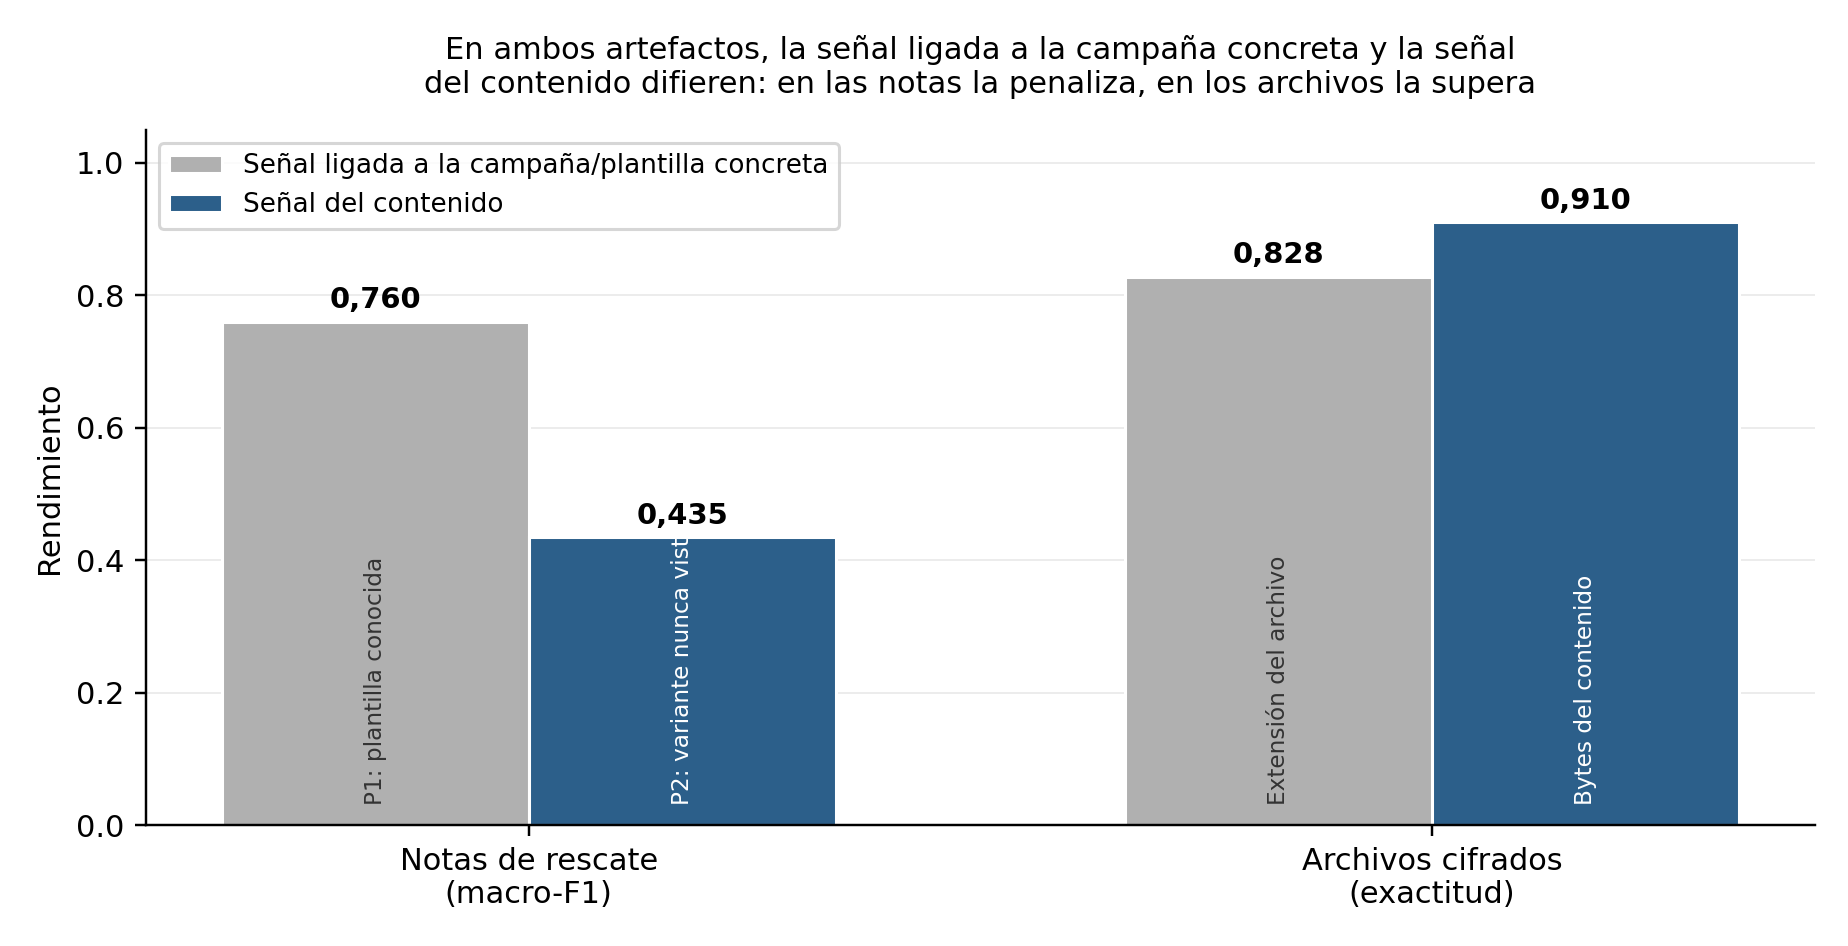
\includegraphics[width=0.92\textwidth]{images/fig_simetria_frentes.png}
\caption{Comparación entre la señal ligada a la campaña o plantilla concreta y la señal del contenido, en los dos artefactos analizados.}
\label{fig:simetria}
\end{figure}

En las \textbf{notas de rescate}, la señal fácil es la plantilla: reconocer una nueva instancia de un texto ya catalogado alcanza un macro-F1 de 0,760, mientras que atribuir una variante nunca vista desciende a 0,435. En los \textbf{archivos cifrados}, la señal fácil es la extensión añadida, que acierta el 100\% de los casos en que está presente pero identifica la campaña y no la familia; la señal de contenido, en cambio, alcanza 0,910 y resulta más estable porque proviene de marcadores que el propio programa escribe en el archivo.

Esta distinción explica por qué las herramientas basadas en catálogos de reglas, como ID Ransomware~\cite{idransomware} o el identificador propuesto por Lemmou et al.~\cite{paper_5_note_files}, funcionan satisfactoriamente sobre campañas conocidas y requieren actualización permanente: operan sobre la señal fácil. Un clasificador entrenado sobre el contenido no las reemplaza, pero cubre el caso que ellas no resuelven, que es precisamente el de las variantes no catalogadas.

\subsection{Implicaciones para el análisis post-ataque}

Los resultados permiten proponer un procedimiento por etapas en el que cada artefacto cumple la función para la que resulta adecuado:

\begin{enumerate}
\item \textbf{Confirmación del incidente} mediante métricas estadísticas sobre los archivos afectados (detección binaria, $\sim$89\% de exactitud). Los archivos cifrados son el único artefacto cuya presencia está garantizada: la nota puede haber sido eliminada, no encontrada, o directamente no existir.
\item \textbf{Identificación de familia por el contenido del archivo cifrado} (91,0\%), aplicable a las 23 familias que añaden estructura reconocible.
\item \textbf{Identificación de familia por la nota de rescate} cuando esté disponible (81,8\% en el escenario comparable con las herramientas existentes), especialmente valiosa para las seis familias que no dejan estructura en los archivos.
\end{enumerate}

\subsection{Sobre la naturaleza de los resultados negativos}

El planteamiento inicial de este trabajo sostenía que las propiedades estadísticas de los archivos cifrados no permiten distinguir familias. La ampliación del espacio de características mostró que esa formulación era demasiado amplia: lo indistinguible es la aleatoriedad del contenido cifrado, no el archivo en su conjunto. Conviene señalar que el resultado negativo original no era erróneo sino insuficientemente delimitado, y que su delimitación precisa ---seis familias de veintinueve--- resulta más informativa que la afirmación general de la que se partió.

Un caso análogo se presenta en el análisis de hiperparámetros de la Sección~\ref{subsec:exp3_hiperparametros}: la ausencia de mejora tras una búsqueda sistemática es en sí misma un resultado, porque desplaza la explicación del rendimiento desde la parametrización del modelo hacia la composición del corpus, que es donde efectivamente se encuentra el factor limitante.

El hallazgo de que las notas de rescate son plantillas de baja variabilidad intra-familia (146 notas, 95 contenidos distintos) reformula el problema de clasificación: el desafío no es distinguir estilos de redacción, sino cubrir el repertorio de plantillas de cada familia. De ahí que el rendimiento bajo P2 esté fuertemente correlacionado con la diversidad de plantillas disponible, y que la expansión del corpus deba priorizarse en \textit{profundidad} (más plantillas por familia) antes que en cantidad de familias.

Finalmente, cabe señalar la importancia metodológica de las métricas elegidas: en un corpus donde dos familias concentran el 25\% de las notas, reportar únicamente accuracy o F1 ponderado sobrestimaría el rendimiento real. La diferencia entre el weighted-F1 (0,798) y el macro-F1 (0,760) bajo P1 ---y la brecha mayor bajo P2 (0,512 vs.\ 0,435)--- ilustra el sesgo que introducen las familias grandes, y justifica la adopción del macro-F1 como métrica principal.

Las limitaciones del estudio son el tamaño del corpus (146 notas, con 7 familias de solo 2 notas), la validación restringida a 2 folds por ese motivo, y la procedencia mixta de las notas (96 archivos brutos, 37 del corpus previo y 13 transcripciones), declarada nota por nota en el manifiesto del corpus.


% ----------------
% -- CONCLUSIÓN --
% ----------------
\chapter{CONCLUSIÓN} \label{chp:conclusion}
\thispagestyle{empty}
\section{Conclusiones Parciales}

Los resultados preliminares obtenidos hasta el momento permiten establecer las siguientes conclusiones parciales:

La detección binaria de archivos cifrados por ransomware mediante métricas estadísticas es viable, alcanzando hasta 100\% de accuracy con modelos basados en árboles de decisión. Esto confirma la efectividad de métricas como la entropía de Shannon, Chi-Cuadrado, estimación Monte Carlo y el coeficiente de correlación serial de bytes para la tarea de identificar si un archivo ha sido encriptado. No obstante, como señalan Lee et al.~\cite{lee2022}, la entropía de Shannon por sí sola no es la métrica óptima y debe combinarse con métricas complementarias para reducir falsos positivos.

La clasificación multiclase de familias de ransomware basada exclusivamente en propiedades estadísticas de archivos cifrados no es viable, alcanzando un máximo del 15,4\% de accuracy sobre 31 clases. Este resultado se explica por la convergencia estadística inherente a los algoritmos criptográficos modernos, que producen salidas indistinguibles entre familias~\cite{paper_4_comparison_of_entropy}.

La evaluación de herramientas existentes revela que las notas de rescate son más discriminativas que los archivos cifrados: ID Ransomware~\cite{idransomware} identifica el 71,93\% de las familias con notas versus el 66,67\% con archivos. Esto motiva el siguiente paso de la investigación.

\section{Trabajo Pendiente}

El trabajo pendiente comprende:

\begin{enumerate}
    \item \textbf{Construcción del corpus de notas:} Recopilar notas de rescate para las 30 familias de NapierOne desde los repositorios ThreatLabz~\cite{threatlabz}, Lemmou~\cite{paper_5_dataset} y fuentes de seguridad públicas, asegurando un mínimo de 2 notas por familia.

    \item \textbf{Clasificación NLP:} Implementar y evaluar el clasificador basado en TF-IDF con n-gramas de palabras y caracteres, comparando LinearSVC, Regresión Logística, Random Forest y KNN.

    \item \textbf{Ejecución en NapierOne-Small:} Repetir los experimentos de clasificación binaria y multiclase sobre el dataset NapierOne-Small (1.000 archivos por familia) para obtener resultados más robustos con las 6 métricas estadísticas completas.

    \item \textbf{Análisis comparativo:} Comparar cuantitativamente la efectividad de ambos enfoques (archivos cifrados vs. notas de rescate) para la identificación de familias.

    \item \textbf{Redacción final:} Completar el capítulo de resultados con los datos experimentales definitivos y las conclusiones finales del trabajo.
\end{enumerate}



% ----------------
% -- REFERENCIAS --
% ----------------
\chapterformattitleonly

\emergencystretch = 1em
\chapter*{REFERENCIAS}
\addcontentsline{toc}{chapter}{REFERENCIAS}
\printbibliography[heading=none]

% --------------
% -- APÉNDICE --
% --------------
\appendix
\chapter*{APÉNDICE}
\addcontentsline{toc}{chapter}{APÉNDICE}
\renewcommand{\thechapter}{A}
%------------------------------------------------------
%------------------------------------------------------

\section{Detección binaria por familia}
\label{apx:binaria_familia}

La Tabla~\ref{tab:apx_binaria_familia} detalla la exactitud de detección binaria (cifrado vs.\ seguro) por familia obtenida con Random Forest en el Experimento~1, referida en la Sección~\ref{sec:exp1}.

\begin{table}[ht]
\centering
\caption{Exactitud de detección binaria por familia (Random Forest)}
\label{tab:apx_binaria_familia}
\begin{tabular}{|l|c||l|c|}
\hline
\textbf{Familia} & \textbf{Exactitud (\%)} & \textbf{Familia} & \textbf{Exactitud (\%)} \\ \hline
WANNACRY & 97,3 & CERBER & 88,7 \\ \hline
CHIMERA & 96,7 & NOTPETYA & 88,7 \\ \hline
MAZE & 96,7 & CLOP & 88,0 \\ \hline
PHOBOS & 96,7 & AVOSLOCKER & 82,7 \\ \hline
BLACKMATTER & 95,3 & CONTI & 82,7 \\ \hline
DARKSIDE & 95,3 & LOCKBIT & 80,7 \\ \hline
BADRABBIT & 94,7 & BLACKBASTA & 78,0 \\ \hline
DHARMA & 94,7 & CUBA & 78,0 \\ \hline
SODINOKIBI & 94,7 & HELLOKITTY & 76,7 \\ \hline
WASTEDLOCKER & 94,7 & SUNCRYPT & 75,3 \\ \hline
CRYPTOLOCKER & 94,0 & NETWALKER & 74,0 \\ \hline
MEDUZALOCKER & 94,0 & RANSOMEXX & 69,3 \\ \hline
RYUK & 93,3 & & \\ \hline
TESLACRYPT & 93,3 & & \\ \hline
BLACKCAT & 92,0 & & \\ \hline
GANDCRAB & 90,7 & & \\ \hline
LORENZ & 91,3 & & \\ \hline
JIGSAW & 90,7 & & \\ \hline
\end{tabular}
\end{table}

\section{Reproducibilidad}
\label{apx:reproducibilidad}

Todas las cifras reportadas en el Capítulo~4 se regeneran a partir de archivos de resultados versionados junto con el código del proyecto: los experimentos 1 y 2 desde \texttt{resultados\_experimentos/}, el experimento 3 desde \texttt{resultados\_canonicos/} (generado por \texttt{clasificador\_notas\_v2.py}, que registra en un manifiesto los parámetros, versiones de librerías y semillas utilizadas), y la evaluación de herramientas desde la planilla de pruebas del proyecto. El corpus de notas cuenta con un manifiesto de trazabilidad que documenta la fuente, el tipo de procedencia y la extensión original de cada nota.


% -----------------------
% -- ÍNDICE ALFABÉTICO --
% -----------------------
\printindex

% -- Ficha Catalográfica --
%\newpage
%\singlespace
%\input{catalografica.tex}
%\onehalfspace

\end{document}
